\documentclass[12pt,oneside,a4paper]{article}
\usepackage{graphicx}
\usepackage{booktabs}
\usepackage{caption}
\usepackage{subcaption}
\usepackage{amsmath}
\usepackage{amsfonts}
\usepackage{amssymb}
\usepackage{lscape}
\usepackage{psfrag}
\usepackage[usenames]{color}
\usepackage{bbm}
\usepackage[update]{epstopdf}
\usepackage[bookmarks,pdfstartview=FitH,a4paper,pdfborder={0 0 0}]{hyperref}
\usepackage{verbatim}
\usepackage{listings}
\usepackage{textcomp}
\usepackage{course}
\usepackage{fancyhdr}
\usepackage{multirow}
\pagestyle{fancy}
\usepackage{tikz}
\usepackage[utf8]{inputenc}
\usepackage[colorinlistoftodos]{todonotes}
\usepackage[version=3]{mhchem}
\usepackage{float}
\usepackage[spanish, es-tabla]{babel}
\setlength{\parindent}{24pt}
\setlength{\parskip}{0.5cm} 

\numberwithin{figure}{section}

\renewcommand{\sectionmark}[1]{\markboth{#1}{#1}}
\renewcommand{\subsectionmark}[1]{\markright{#1}}

\fancyhf{}
\fancyhead[RO]{\nouppercase{\footnotesize\sc\leftmark\ \hrulefill\ \thepage}}
\fancyhead[RE]{\nouppercase{\footnotesize\sc\thepage\ \hrulefill\ }}
\renewcommand{\headrulewidth}{0pt}

\makeatletter
\def\cleardoublepage{\clearpage\if@twoside \ifodd\c@page\else%
\hbox{}%
\thispagestyle{empty}%
\clearpage%
\if@twocolumn\hbox{}\clearpage\fi\fi\fi}
\makeatother


\renewcommand{\topfraction}{0.9}  % max fraction of floats at top
\renewcommand{\bottomfraction}{0.8} % max fraction of floats at bottom
% Parameters for TEXT pages (not float pages):
\setcounter{topnumber}{2}
\setcounter{bottomnumber}{2}
\setcounter{totalnumber}{4}            % 2 may work better
\setcounter{dbltopnumber}{2}           % for 2-column pages
\renewcommand{\dbltopfraction}{0.9}    % fit big float above 2-col. text
\renewcommand{\textfraction}{0.07}     % allow minimal text w. figs
% Parameters for FLOAT pages (not text pages):
\renewcommand{\floatpagefraction}{0.7}  % require fuller float pages
% N.B.: floatpagefraction MUST be less than topfraction !!
\renewcommand{\dblfloatpagefraction}{0.7} % require fuller float pages

\sloppy

\widowpenalty=10000
\clubpenalty=10000

\edef\today{%\number\day\
\ifcase\month\or
January\or February\or March\or April\or May\or June\or July\or
August\or September\or October\or November\or December\fi\ \number\year}
\title{\vspace*{40.0mm}
  \bf\sf ALERGIAS Y POLEN
         \vspace*{20.0mm} \\
  \vspace*{40.0mm}
  %\vspace{-20mm}\framebox{DRAFT VERSION}\vspace{20mm} \\
  \Large\bf\sf Los Físicos Valen Para Todo S.A. \vspace*{20.0mm}}
\author{\sf }
\date{\sf 17 de marzo de 2015}

\begin{document}

\begin{figure}
  \parbox[t]{125mm}{
    \vspace*{6mm}
    \scriptsize\sf           UNIVERSIDAD DE CANTABRIA\\
    \scriptsize\sf           FACULTAD DE CIENCIAS\\
    \scriptsize\sf           DEPARTAMENTO DE FÍSICA \\
    \scriptsize\sf           LOS CASTROS, S/N, 39005 SANTANDER\\
    \scriptsize\sf\bfseries  PROYECTOS: concepción, desarrollo y herramientas\\
    \scriptsize\sf\bfseries  TIPO DE PROYECTO: \textit{e-ciencia}}
  \parbox[t]{40mm}{
    \begin{flushright}
      
\includegraphics[height=25mm]{UC.jpg}
    \end{flushright}}
\end{figure}

\maketitle
\thispagestyle{empty}
\raggedbottom

\cleardoublepage
\pagenumbering{roman}
\setcounter{tocdepth}{2}

\vspace*{\fill}
\section*{Resumen}
La alergia al polen es un problema para 6 millones de personas en toda España que resurge periódicamente cada primavera. Si bien existen estudios que miden las concentraciones de polen continuamente, así como estudios históricos sobre los periodos en los que cada especie vegetal florece y produce polen, no existe ninguna forma de predecir estos comportamientos de forma suficientemente precisa y ajustada a las circunstancias climáticas que van teniendo lugar a lo largo del año. El proyecto \textit{Alergias y polen} tiene como objetivo precisamente la predicción de las concentraciones de polen con precisión de un día, de una forma similar a la predicción del tiempo meteorológico. Esto permitiría a las personas afectadas con esta enfermedad tomar precauciones en los días con mayor concentración polínica. Para lograr este objetivo, se propone realizar observaciones fenológicas de las especies cuyo polen es causante de alergias (principalmente oleas y gramíneas) mediante cámaras instaladas en las propias plantaciones, que serán acompañadas con predicciones meteorológicas para estudiar la variación de la producción polínica y predicciones de propagación de partículas para estudiar su difusión en el aire.


\section*{¿Quiénes somos?}

El grupo \textit{Los Físicos Valen Para Todo SA} está formado por un conjunto de aventajados estudiantes del último año del Grado de Física de la Universidad de Cantabria. En nuestro grupo destacan la ética de trabajo y la implicación de todos los componentes, así como la juventud de los mismos, lo cual ayuda a generar un ambiente de trabajo agradable e inspirador a la par que serio y disciplinado. Asimismo, nuestra corta edad e inexperiencia nos convierte en un grupo emprendedor con voluntad tenaz y determinación firme para contribuir a la sociedad y abrir nuestro propio camino en el mundo de la ciencia y la tecnología.

\vspace*{\fill}
\cleardoublepage

\section*{Resumen ejecutivo}

Desarrollar un modelo para la predicción de la concentración de polen en el aire y conocer cómo se distribuye por la región de Andalucía es un proceso que requiere una planificación detallada, a través de la cual se pueden obtener resultados importantes para la mejora de la calidad de vida de la población alérgica. Para ello, se va a realizar un seguimiento del florecimiento de diferentes plantaciones mediante el estudio de la meteorología y la instalación de fenocámaras y captadores de polen.

En primer lugar, es necesario conocer la meteorología del lugar para conocer cómo influye la temperatura o el volumen de las precipitaciones en una región determinada en el florecimiento de los olivos, y poder predecir hacia dónde llevará el viento los granos de polen.  

La instalación de fenocámaras permitirá tomar imágenes y realizar un seguimiento diario del estado de las plantaciones. Para ello, las cámaras se instalarán en las principales plantaciones de olivos, trigo y encinas. El conjunto de datos, en forma de imágenes, serán analizados en dos fases: una primera informatizada, que consistirá en la elección de las imágenes que posean información útil; y una segunda fase humana, en la que un técnico seleccionará las fotografías que poseen información importante.

Además de las fenocámaras, se utilizarán captadores volumétricos de partículas que permitirán medir la concentración de polen en el aire en un lugar determinado. Uniendo los datos obtenidos mediante estos dos procesos, se realizará una base de datos que se actualizará diariamente.

El producto final de este proyecto será un software informático, escrito en el lenguaje FORTRAN, capaz de elaborar una predicción totalmente fiable de la concentración de polen en las diferentes zonas de Andalucía.  Al final se dispondrá de 6 pequeños módulos independientes de simulación de concentración, que se encargarán de cuantificar el efecto de cada uno de los factores que intervienen en la concentración de polen en el aire. Estos módulos pueden ser reutilizados o revendidos según sea conveniente. 

Con el fin de verificar la calidad del modelo, se someterá el software a varios procedimientos de prueba durante su desarrollo. Para facilitar la flexibilidad y adaptación se realizarán simulaciones con la utilización de datos históricos en este campo, lo cual permitirá realizar estudios con diferentes tipos de clima, depurando al máximo posible la respuesta del programa. Por último, durante el transcurso de estas simulaciones, se hará un estudio paralelo en el cual se discierna claramente si el modelo final es aplicable únicamente a Andalucía, o si es posible realizar modificaciones leves y convertirlo así en adaptable a otras regiones. 

\cleardoublepage

\tableofcontents
\cleardoublepage
\pagenumbering{arabic}

\cleardoublepage

\section{Introducción}

La alergia es un proceso autoinmune, una reacción excesiva del sistema inmunológico ante sustancias exteriores al cuerpo que se denominan alérgenos. Desde el momento en que nacemos, nuestro sistema inmune tiene que aprender qué puede considerarse como dañino y qué no, ya que carece de la capacidad de reconocer de manera innata los gérmenes. Curiosamente, de manera general, una persona no desarrolla alergia al polen hasta la edad de cinco o seis años y, realmente, no se conoce una teoría de por qué lleva 5 o 6 años desarrollar una alergia. En el caso de la alergia al polen, ésta se desarrolla cuando el individuo ha padecido una enfermedad vírica. Existen pruebas que muestran que los niños infectados con virus que afectan la nariz y los pulmones tienen a su vez una mayor exposición a alérgenos como el polen, lo cual es el origen de la alergia. Hay múltiples tratamientos para curar o tratar las alergias: antihistamínicos, corticoides, adrenalina y broncodilatadores.

Uno de los principales causantes de alergias, como se ha resaltado anteriormente, es el polen. El polen son granos de tamaño microscópico. Son producidos por el aparato reproductor masculino de las flores y portan las células espermáticas hasta el aparato reproductor femenino para fecundarlo. Una sola planta puede producir miles de granos de polen, que se ve como polvo amarillo en las flores pero que no puede verse cuando está disperso en el aire. La producción polínica varía a lo largo del año, teniendo lugar la máxima producción en primavera. Existe una variedad muy amplia de tipos de polen, si bien los principales causantes de alergias son los provenientes de las gramíneas y las oleas (olivo, por ejemplo).

 
Para predecir la producción de polen se realizan observaciones fenológicas de las plantas. La fenología es la ciencia que estudia los procesos biológicos en función de diversos factores como los periodos estacionales, el clima o la deriva del tiempo atmosférico (temperatura, humedad, régimen de lluvias, etc.) a lo largo de un año en un cierto lugar. Dichos procesos biológicos incluyen ciclos de plantas e insectos, cambios en árboles y arbustos (caída de hojas o cambios de color), migraciones de aves u otros animales... Nos centraremos en los ciclos (de floración, específicamente) de las plantas debido a que la producción polínica que nos interesa es función de ellos. Además, observando el estado fenológico de una planta se pueden prever su futura evolución fenológica.

En lo relativo a nuestro caso, focalizaremos nuestra atención concretamente en la fenología de las tres especies vegetales que afectan al tema en cuestión de las alergias al polen en un grado mayor: las oleas (concretamente el olivo), gramíneas y quercus (roble y encina). En la sección de Referencias se pueden encontrar gráficos de producción polínica de estas y otras especies en Jaén [\ref{ref:calen_J}], Almería [\ref{ref:calen_A}] y Granada [\ref{ref:calen_G}]. También un mapa de la distribución de diferentes especies en Andalucía en [\ref{ref:especies_andalucia}].
 
En primer lugar, el olivo tiene un periodo de floración corto cuya mayor actividad se encuentra desde abril hasta junio, alargándose hasta principios de octubre con baja actividad [1][2][3]. Es precisamente por esto que su producción polínica es elevada, lo que, teniendo en cuenta la gran cantidad de cultivos de esta especie, aumenta muy significativamente la concentración de polen durante estos meses. Este período llega a su fin cuando las flores pierden sus pétalos y surge el fruto, la aceituna, en un proceso que se denomina cuajado. La clave fenológica utilizada en la observación del olivo es la propuesta por Maillard (1975).

\begin{figure}[H]
\begin{center}
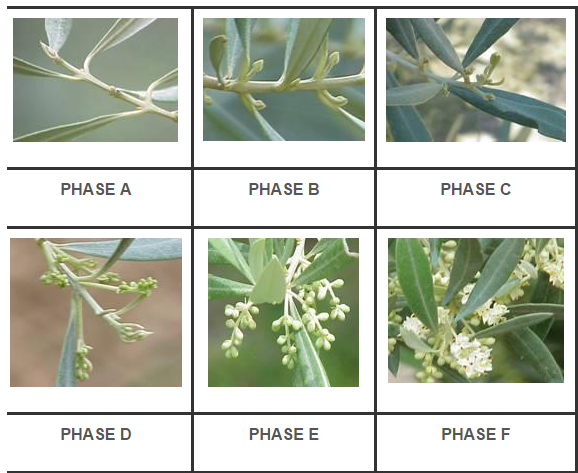
\includegraphics[scale=.7]{clave_olivo.png}
\caption{Clave fenológica de olivo por Maillard (1975). [\ref{ref:uco1}]}
\label{fig:clave_olivo}
\end{center}
\end{figure}

Por su parte, las gramíneas comprenden un amplio grupo que incluye formaciones herbáceas, los extendidos plumeros (cortadeira selloana) o cultivos de secano como el trigo. Su periodo de floración es más largo que el de los olivos pero también más suave, y abarca desde febrero hasta principios de octubre [\ref{ref:uco1}][\ref{ref:uco2}][\ref{ref:uco3}]. Se puede encontrar un mapa de distribución de gramíneas en Andalucía en [\ref{ref:gram_andalucia}], así como de campos de cultivos de secano (trigo) en [\ref{ref:trigo_andalucia}]. La clave fenológica es la propuesta por Prieto-Baena (2004) donde se tiene en cuenta el porcentaje de apertura de flores por espiga.

\begin{figure}[H]
\begin{center}
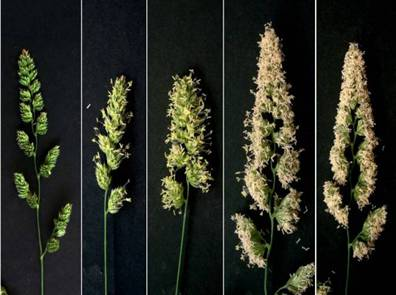
\includegraphics[scale=.8]{clave_gram.jpg}
\caption{Clave fenológica de gramíneas de Prieto-Baena (2004). [\ref{ref:uco2}]}
\label{fig:clave_gram}
\end{center}
\end{figure}

Estas dos especies son, como se ha visto, las dos mayores causantes de alergias y por lo tanto serán en las que centremos nuestro estudio. No obstante, la floración de las gramíneas, como se puede observar en la Fig. 2, no es muy viva. Esto hace que su observación por métodos a distancia sea difícil, por lo que se requieren otros métodos para controlarla. Como se puede observar en [\ref{ref:uco1}][\ref{ref:uco2}][\ref{ref:uco3}], el término de su periodo de floración coincide con el del olivo, mientras que el comienzo coincide con el del quercus. La familia quercus comprende la encina y el roble y su período de floración comprende desde finales de febrero hasta junio o marzo, siendo bastante intenso desde el principio, lo que permite una buena observación de su comienzo, especialmente en la encina, cuyas flores son fácilmente visibles.

\begin{figure}[H]
\begin{center}
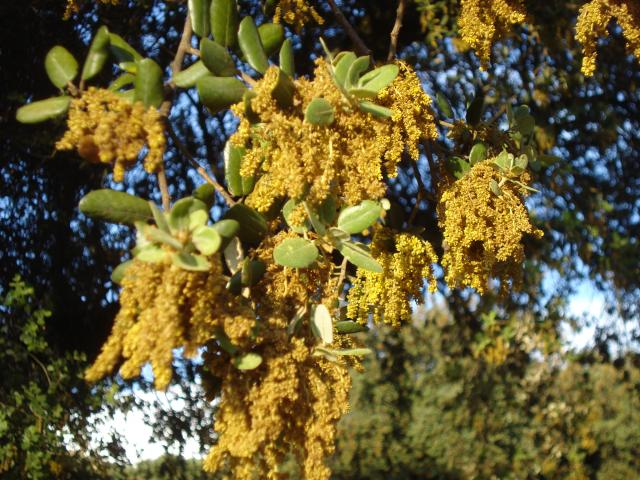
\includegraphics[scale=.3]{flor_encina.jpg}
\caption{Flores de encina. [\ref{ref:flor_encina}]}
\label{fig:flor_encina}
\end{center}
\end{figure}

Las flores, tanto del olivo como de la encina, pueden ser observadas mediante fenocámaras instaladas en las propias plantaciones para monotorizar los cambios fenológicos a una escala de tan sólo horas.

Por otro lado, existen diferentes captadores y aparatos de medida de concentraciones de polen, dependiendo del tipo de medida que se quiera realizar: de muestreos continuos o cortos de la atmósfera, según períodos estacionales, de contaje de partículas en aire, etc. Los dispositivos que miden la concentración de polen se basan en diferentes métodos de captación: basados en gravedad, que constan de superficies adhesivas que recogen los precipitados del aire por efecto de la gravedad; basados en impacto, que aprovechan la inercia de las partículas para que impacten sobre sustancias adhesivas; o basados en filtración, que se basan en la capacidad de filtración de las partículas. Cabe destacar dos tipos de captadores: el captador Cour (medidas semanales) y el captador Hirst (medidas horarias o diarias). El captador Hirst es el más extendido en Europa y es el modelo utilizado por la Red Española de Aerobiología  para el registro continuo de partículas de la atmósfera y la recogida de polen y esporas. Los dispositivos son delicados, por lo que no se pueden utilizar de cualquier manera y requieren de una serie de adaptaciones tanto en su ubicación como previas a su puesta en marcha.

Finalmente profundizaremos en el aspecto relativo al clima, que, como ya se ha comentado, tiene una gran influencia en la floración y la producción de polen, pero también lo tiene en su propagación. Estudiarlo nos aporta información de cómo éste afecta a la producción y distribución del polen, y permite establecer unas bases y estimaciones \textit{grosso modo} para prever el efecto de éstos en los potenciales casos de alergias que sufra la población de estudio. Dado que este proyecto va a ser llevado a cabo en Andalucía, nos interesa tener datos sobre el clima en las distintas regiones que componen la Comunidad Autónoma, que están resumidos en la siguiente tabla.

\begin{figure}[H]
\begin{center}
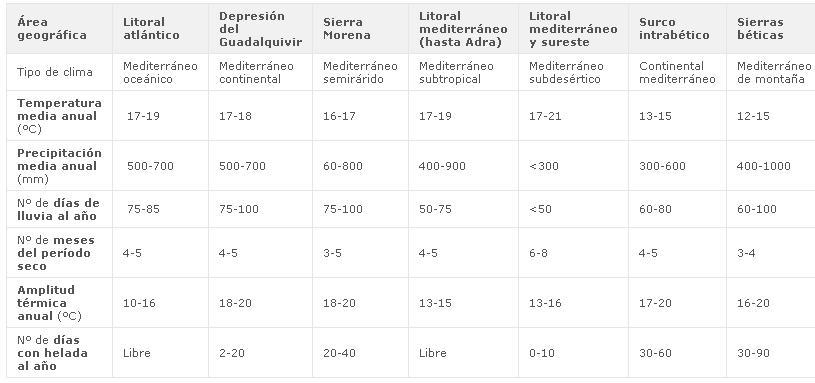
\includegraphics[scale=.7]{tabla_clima.JPG}
\caption{Tabla que recoge los diferentes tipos de clima de Andalucía. [\ref{ref:junta_andalucia}]}
\label{fig:tabla_clima}
\end{center}
\end{figure}

El clima tiene a su vez una gran influencia sobre la meteorología de una región. La meteorología es un concepto más específico y nos permite obtener con un mayor detalle los modelos de propagación y producción de polen, ya que tiene una influencia más evidente en el ciclo de producción y de floración.

Los factores meteorológicos afectan de forma diferente dependiendo del punto en el que nos encontremos dentro del ciclo fenológico de floración de las plantas. Los efectos pre-floración se estudian de manera que si una planta tiene una floración típica en abril, los eventos condicionantes más importantes se producen en febrero y marzo, mientras que lo ocurrido, por ejemplo en octubre, tiene una importancia marginal en comparación. Los efectos de los agentes meteorológicos durante la época de floración presentan efectos más inmediatos, siendo necesario predecir el comportamiento de estos agentes para poder predecir la evolución de los niveles de polen. Es decir, una vez ha ocurrido un evento meteorológico el tiempo de reacción y de previsión antes de que el efecto en los niveles de polen sea apreciable, es mínimo e incluso inexistente en muchos casos. Por eso es de vital importancia conocer cómo se relacionan estos procesos con los niveles de polen, de forma que la predicción meteorológica pueda llevar asociada una predicción fiable de niveles de polen. 

Como se ha podido ver hasta ahora, hay gran cantidad de factores que influyen en la producción y propagación de polen, pero a la hora de cuantificar la concentración de polen en el aire el factor más importante es el número de focos emisores que se encuentran próximos al lugar de estudio. A partir de ahí, conocer cómo se produce la propagación del polen en el ambiente es de vital importancia para la prevención y tratamiento de alergias, ya que el polen es producido por plantas que en su mayoría no se encuentran dentro de los núcleos urbanos.

Los principales mecanismos de propagación y difusión del polen se producen, o bien mediante el aire (mecanismo anemófilo) o mediante la intervención activa de agentes propios del ecosistema en cuestión, como pueden ser animales o en particular los insectos (mecanismo entomófilo). Cada propagación se corresponde, principalmente con el tipo de planta y se puede relacionar con las características de los granos de polen. 



\section{Desarrollo del modelo}

El modelo busca la predicción de la concentración del polen en el ambiente en la región de Andalucía. Para ello será necesario controlar tres factores: primero la toma de medidas de la concentración de polen en el aire, segundo el seguimiento del florecimiento de plantaciones de olivos y gramíneas mediante fotografía; y por último disponer de una serie de datos meteorológicos.

Es necesario mencionar que no vale que los datos sean solo a tiempo real sino también pasados y futuros, por dos razones:

- La raíz del modelo busca una combinación entre el florecimientos de las plantas y la meteorología, y para encontrarla hacen falta datos históricos.

- El funcionamiento del modelo busca la predicción de la concentración de polen en aire, así que es obvio necesitar datos de predicciones meteorológicas.

\subsubsection{Opción 1: Toma de fotos mediante satélite}

Una estimación de la cantidad de fotos en las que se podría apreciar el florecimiento de los olivos sería la siguiente:

La región de Andalucía tiene una superficie de 87268 km$^2$ en las cuales se registró una población de olivos de 174,78 millones en 2013. Esto hace que ocupen una superficie de 14.790 km$^2$. Se dispondría de un satélite que tome imágenes de 10,15 x 10,15 km y que posee una resolución espacial de 5,8 metros en banda multiespectral para así poder detectar las manchas blancas de las flores del olivo. Según esta medida sería necesaria la toma de 848 fotos para cubrir todo el área de Andalucía.

El aspecto positivo de la toma de fotos mediante satélite es que el periodo de revisita es de 3 a 5 días, ya que la flor del olivo se hace visible a mediados de mayo con variaciones dependientes del lugar de cultivo, la variedad o el año. Su duración no viene a pasar más allá de una semana, aunque desde que se abre la primera flor hasta la última en un mismo olivo puede pasar un tiempo de hasta tres semanas. Durante ese tiempo el polen que es vertido a la atmósfera es muy elevado en comparación a otras plantas, siendo el aire el encargado de dispersar las partículas. La toma de fotos se realizaría cada periodo satelital desde el mes de Marzo hasta junio (durante 3 años) ya que son los meses en los que florece el olivo y el resto de meses se obtendrían fotos semanales cada 6-10 días (dos períodos satelitales). Un ejemplo de satélite que puede proporcionar estas medidas es el FASat-Charlie (SSOT), aunque el siguiente enlace aparecen un conjunto de satélites más [\ref{ref:Charlie}].

\subsubsection{Opción 2: Toma de fotos mediante cámaras \textit{in situ}}

Se ha comentado ya la posibilidad de medir el estado de floración de gramíneas y olivos a través de cámaras instaladas en las propias plantación de estudio. Para llevar esto a cabo sería necesario no solo localizar las principales plantaciones de olivos y gramíneas sino también desplegar en ellas una red semi-autónoma de cámaras conectadas con un servidor central de forma que el proceso de toma y recogida de fotos se realice sin intervención humana directa.

En cuanto al estudio de olivos es fácil controlar las principales plantaciones, puesto que los olivares más importantes están catalogados y son propiedad de alguna persona/empresa que los usa para su explotación comercial. Sin embargo el caso de las gramíneas es mucho más complejos ya que, a excepción del trigo (que sigue un patrón similar al del olivo), las gramíneas se encuentran distribuidas uniformemente por el territorio lo que sumado a la escasa visibilidad de sus flores hace casi imposible un seguimiento. Como solución a este problema se propone el estudio de la familia $Quercus$, en concreto de las encinas. Estas plantas tienen una fenología levemente más temprana que las gramíneas, por lo que puede servir como estimación predictiva de éstas. Asimismo, cabe recordar que el olivo y las gramíneas tienen una etapa de floración similar por lo que a partir de los datos de una especie se puede inferir el estado fenológico de la otra, siempre que se encuentren en una zona meteorológicamente similar o equivalente.

Se debe contar con un software de análisis de imágenes para detectar si la plantación en cuestión ha florecido o no. La opción más interesante, debido a las limitaciones de precisión de este tipo de softwares, se prevé que sea el uso conjunto de éste y análisis humano. De esta forma el software se configuraría como filtro grueso para reducir la carga de trabajo de la persona encargada de determinar, sobre las fotos que pasen el filtro del software, si existe o no floración.

Este método presenta una serie de inconvenientes respecto a la toma de datos mediante satélites como son la cantidad de fotos necesarias (en torno a 2000-3000) y el coste temporal/económico de su instalación, además de las tarifas de conexión a Internet asociadas con la necesidad de enviar las fotos a un sistema centralizado. A todo esto deben incluirse los problemas derivados de la utilización de hardware instalado en las propias plantaciones como, por ejemplo, los robos.

Sin embargo, la detección mediante este tipo de cámaras ofrecen grandes ventajas como es el control directo por parte de la empresa, la posibilidad de aumentar la cantidad de fotografías tomadas dependiendo de la estación fenológica (no hay que esperar a que el satélite vuelva a pasar por la zona de estudio), además de mejorar las condiciones de toma de imágenes mediante la colocación de fondo de alto contraste detrás de las zonas a fotografiar, aumentando la eficiencia del sistema.

Es por esto que para la realización de este proyecto concreto se ha escogido la instalación de cámaras en las plantaciones y zonas de control. Se apuesta por tanto por un proyecto que dependa lo menos posible de terceros y que sea capaz de funcionar de la forma más eficiente y autónoma. Además a largo plazo se ha estimado un ahorro económico supeditado a que las estimaciones de robos y fallos en las cámaras instaladas se ajusten a la realidad.

\subsubsection{Datos de la concentración de polen en el aire}

A través del uso de un sistema que nos permita detectar la concentración de partículas de polen y esporas en el aire, se creará una base de datos. Para ello se va a utilizar un captador de partículas volumétrico por succión, que permite obtener datos homologables independientemente de las características biogeográficas y bioclimáticas de la zona. El caudal de succión de estos captadores es de 10 litros de aire/min, similar al volumen de inhalación de aire por el pulmón, y deberán colocarse en una superficie horizontal, a una cierta elevación, evitando un posible apantallamiento por edificios colindantes u otros obstáculos. Las medidas que se van a efectuar con este aparato se realizarán durante todas las horas del día, en un principio durante un periodo de dos años. Pasado este periodo inicial de toma de datos, en los 3 años posteriores, las medidas se realizarán 3 días a la semana, menos los meses de marzo a junio que se volverá a una medición diaria. Para validar los datos obtenidos en el estudio, serán contrastados con datos de años anteriores en este campo, realizados por la Universidad de Córdoba u otras con las que se debe iniciar un contrato. En el siguiente enlace [\ref{ref:metodologia}] se puede ver el proceso de toma de datos.


\subsubsection{Datos meteorológicos}

Para conocer cómo y cuándo se reparte el polen por la región de interés es necesario conocer la meteorología del lugar. Esto incluye la medida de la propagación del viento, la temperatura y la lluvia. El primero porque es el encargado de esparcir el polen y los segundos porque afectan de forma directa a la fenología del lugar. En cuanto a los datos meteorológicos históricos de Andalucía, se tomarán los datos desde el año 2010 hasta 2017. Los datos correspondientes al periodo desde 2010 hasta 2015 se usarán para desarrollar el modelo y los dos años restantes (2015-2017) para comprobar si realmente el modelo funciona. La toma de estos datos no conlleva ningún problema, ya que AEMET dispone de datos meteorológicos desde 1950.

\subsubsection{Obtención de fotos mediante la organización de un sorteo}

Con el fin de obtener un número mayor de fotos cuando los olivos florezcan en el año 2017, se ha contemplado la realización de un sorteo para la campaña primavera/verano del 2017. El mecanismo consiste en la creación de una plataforma en la página web donde fotógrafos aficionados (o cualquier individuo con una cámara en su teléfono móvil) puedan subir fotos de los olivos en flor. Cada foto seleccionada se pagará a 0.50 céntimos siempre que cumpla una serie de requisitos que serán especificados cuando se establezcan las bases del sorteo (uno de los requisitos será, por ejemplo, que la foto enviada sea la primera en ser recibida de una zona concreta). Las tareas correspondientes a la gestión del sorteo serán competencia del WP9. El incentivo final para obtener la ayuda desinteresada de estos fotógrafos amaetur será el sorteo (en verano del 2017) de una PlayStation 4 (recogida en el WP2) entre los individuos cuyas fotos fueron seleccionadas. 

\subsection{Producto}

El producto será un software informático capaz de, a partir de los datos actuales de meteorología, concentración y estado de los focos principales de polen (fotografías \textit{in situ}), elaborar una predicción realista de los niveles de polen esperados para el siguiente día (2 sigmas de confianza) y una estimación para los siguientes 7 días naturales (1 sigma de confianza) a escala local.

\subsubsection{Detalles generales del producto}

Se ha escogido FORTRAN como lenguaje de trabajo (aunque no es necesariamente una decisión final) por su eficiencia y sencillez que hacen no sólo rápida su ejecución en cualquier ordenador, sino que ademas permite un aprendizaje relativamente rápido. Además, FORTRAN es un lenguaje muy extendido tanto fuera como dentro del ámbito de la ciencia lo que facilitará la posible reutilización de un código ya existente.

El esquema del programa será orientado principalmente a la modularidad. De esta forma se dispondrá lo antes posible de pequeños módulos independientes de simulación de concentración de polen que puedan ser reutilizados o revendidos según sea conveniente. El software contará con 6 (4 + integración y GUI) módulos de simulación, que se encargarán de cuantificar el efecto de cada uno de los factores claves que afectan a la concentración de polen en el aire. Se trabajará la integración de los mismos incluyendo el reparto de los datos pertinentes (el programa lee todos los datos y selecciona cuál corresponde a cada módulo), la recogida, y combinación racional de todas las predicciones, así como la salida final de los datos sobre concentración de polen en cada zona. Además, se introducirá como extra y valor añadido al producto, una interfaz gráfica que permita un control sencillo del software de forma que sea posible su utilización sin a penas aprendizaje previo. En cualquier caso se crearán tanto una extensa documentación sobre el funcionamiento del programa como un manual de uso rápido para facilitar el acceso a personal inexperto.

\subsubsection{Componentes del producto}

Dentro de cada uno de los módulos se llevarán a cabo una serie de tareas similares, sin un esquema temporal estricto ni prefijado, dejándose total libertad interna de organización, aunque siempre dentro de los plazos y cumpliendo los requisitos necesarios para conseguir un programa con un funcionamiento satisfactorio. Estas tareas incluirán el análisis de los datos pasados, la elaboración de un modelo sencillo de correlación entre el factor de estudio y la concentración de polen, y la implementación de dicho modelo (y cualquier corrección que pueda ir surgiendo durante el proceso) en código FORTRAN estable, sin fallos y eficiente.

Los módulos se dividirán entre los diversos factores climáticos que se estudiarán, a saber, los ya mencionados viento, precipitaciones, temperatura (aunque podrían surgir más). Cada módulo pasará por una serie de fases con una estricta organización temporal y unas fechas de entrega marcadas. Las fases del desarrollo del programa serán denominadas: Alpha, Beta, RC (Release Candidate) y FR (Final Candidate) adecuándose a la nomenclatura tradicional en desarrollo de Software.

En la fase Alpha cada módulo trabajará por separado compartiendo únicamente la información necesaria para la integración posterior. Al terminar esta fase todos los módulos deberían funcionar correctamente por separado y ser capaces de hacer predicciones razonables en el caso ideal de que solo uno de los factores existiera. En la siguiente fase, la fase Beta, se trabajarán la integración e intercomunicación necesaria de todos los módulos, así como una versión sencilla y prototípica de lo que será la GUI; al terminar esta fase debería disponerse de un software capaz de realizar unas predicciones razonables con un número de fallos pequeño, aunque no necesariamente inexistentes. Se comienza entonces la fase RC en la que se trabaja puliendo los modelos (en la eventualidad no deseable pero posible de que hiciera falta), se mejorará también la integración y se corregirán todos los fallos encontrados en esta, así como se realizará la GUI definitiva con la que se podrá interaccionar con el programa. Al concluir esta fase debería tenerse una versión entregable del sistema completo incluyendo no solo predicciones sino GUI. El software será posteriormente verificado y testeado, con muestras aleatorias de los datos (muestra preseleccionada y que se omitió a propósito de los datos empleados en la elaboración del modelo), así como al menos un año de los datos más recientes.

Cualquier fallo que se produzca en esta etapa debe ser identificado y corregido a fin de presentar una versión final FR libre de \textit{bugs} y errores, y que ha pasado satisfactoriamente gran cantidad de pruebas.

Durante todo el proceso de desarrollo del software se hará especial hincapié en la elaboración de una buena documentación del programa así como la elaboración del 'Manual de uso rápido' que se pueda distribuir con el producto final a cualquier comprador.

Uno de los objetivos del software y de la decisión de optar por un modelo altamente modular es la posibilidad de reutilizar todo el software realizado en cualquier punto del desarrollo. De esta forma, además de la entrega a la Comunidad de Andalucía se puede vender el software entero o por módulos a cualquier comprador interesado en un modelo de simulación de polen en función de la floración y la meteorología. Además el programa es susceptible de reciclarse como modelo de simulación de concentración de cualquier tipo de partícula en suspensión, como contaminantes producto de las centrales térmicas, mediante unos reajuste en el código.

\subsubsection{Funcionamiento del software}

Al software se le proporcionarán datos meteorológicos más recientes así como las concentraciones de polen más actuales en el momento de ejecución. También requerirá la localización y estado de floración de los principales focos de polen (gramíneas y olivos). El programa calculará entonces la concentración futura de polen en las zonas deseadas con los valores de precisión antes mencionados. Para asegurar una recogida de polen eficiente y constante, así como una información actualizada y fiable sobre el estadio de floración de los principales focos, el proyecto recoge la implantación de varios centros y detectores en los que se recogerán las muestras de polen y se analizarán las imágenes de los focos de floración.

Tanto la introducción como la salida de datos se realizarán de acuerdo con un formato a consensuar con las partes implicadas. El control del programa se podrá realizar tanto por línea de comandos como mediante la interfaz gráfica que se provee con el producto final.

Para la realización de la simulación se prevé la utilización de un ordenador comercial de alto rendimiento, un gran \textit{cluster} de computación o algún tipo de hardware similar con gran poder de cálculo. Así mismo se propone realizar una simulación diaria en el caso ideal y se recomienda no menos de 3 por semana para garantizar resultados satisfactorios.

\clearpage

\textbf{Recursos:}

\begin{itemize}
\item Recursos destinados a la toma de datos.
\item Personal y equipo:
\begin{itemize}
\item Personal necesario para desarrollar y testear el software, formado por programadores y expertos en el análisis de datos medioambientales: 3-4 personas.
\item Personal encargado del mantenimiento: técnicos que se encarguen del correcto funcionamiento del programa y den mantenimiento periódico al sistema. (En este punto es necesario saber el número de estaciones que se van a colocar, si el soporte es global o local, etc.). Este tipo de técnicos necesita una formación previa para realizar correctamente esta tarea.
\item Coordinador encargado de contactar y gestionar las relaciones con agencias y organizaciones que suministren datos o colaboren en el proyecto (AEMET, Junta de Andalucía, universidades...).
\item Hardware necesario para ejecutar el modelo, así como el tipo de instalación en el cual se situará el equipo que trabaje con el mismo.
\end{itemize}
\end{itemize}

\subsubsection{Detalles del producto terminado}

El producto final que se entregará al cliente será un software con su correspondiente documentación y manual de uso. Además el proyecto desarrollado para la Comunidad de Andalucía incluye la creación de varios centros de control de la concentración del polen y la floración de gramíneas y olivos mediante fotografía "\textit{in situ}” y un equipo de mantenimiento del software.


\subsection{Verificación}

Con el fin de verificar la calidad y el correcto funcionamiento del modelo, se someterá a varios procedimientos de verificación durante su desarrollo.

\subsubsection{Simulaciones comparativas respecto a otros años}

Obteniendo los datos cronológicos de la concentración de polen en la Comunidad Autónoma a través de estudios o ciertos organismos (las Universidades de Córdoba o Granada realizan este tipo de estudios), se realizará un testeo del software introduciendo esta información y comprobando si los resultados son acordes a los patrones esperados. Esta metodología también permitirá optimizar la flexibilidad y adaptación del modelo, proporcionando datos de distintos tipos de clima y depurando su respuesta lo máximo posible en función de qué parámetros sean relevantes, el tipo de vegetación del cual disponga la zona...etc.

Otra opción interesante es realizar estas simulaciones de forma modular, analizando por separado cómo intervienen las diferentes variables, para posteriormente integrar todos los datos y crear un modelo en el que todo converja para expresar el resultado final. Este procedimiento asegura una rápida detección de errores y permite trabajar con varios módulos en paralelo.

Por último, se hará un estudio a la par que estas simulaciones en el cual se delimite claramente si el modelo final es aplicable únicamente a Andalucía, o si es posible realizar modificaciones leves y hacerlo adaptable a otras regiones, con el fin de conseguir un modelo mucho más global y con futuro más allá de este proyecto.

\subsubsection{Comprobación de que el modelo funciona y es consistente}

Una vez puesto a punto el software, se deben comenzar las pruebas reales sobre el terreno. Para verificar estos resultados, se utilizarán principalmente dos fuentes:

\begin{itemize}
\item \textit{Agencias que hagan este mismo trabajo y posean una página web.} Por ejemplo en la Universidad de Granada, Jaén y Almería se controla periódicamente la concentración de polen y la previsión de la misma en dichas comunidades [\ref{ref:ugr}]. Contrastando sus datos con los que se obtengan en este modelo se puede certificar la viabilidad de nuestro software para esas regiones.
\item \textit{Establecer plantaciones de control cuya información de polinización sea conocida} y comprobar que nuestro modelo determina y predice correctamente los datos que se obtendrán de dicha plantación por otros métodos, como puede ser el tradicional análisis con una estación de filtrado de aire y microscopía óptica. Este tipo de instalaciones idealmente deberán localizarse en todas las áreas de Andalucía que tengan un tipo de clima distinto y unas condiciones meteorológicas concretas y relevantes que influyan en la propagación del polen (fuertes vientos, gran humedad) o cerca de núcleos de riesgo como pueden ser grandes ciudades.
\end{itemize}

\subsubsection{Controles de mantenimiento y calidad}

Una vez realizadas todas estas pruebas y lanzado el producto, éste ha de ser sometido a revisiones periódicas con el fin de controlar que los datos proporcionados sigan siendo fiables, que el software funciona sin problemas, e incluso si es susceptible de ser mejorado gracias a nuevos avances en el campo de la programación o en la formación del personal responsable de operar con este modelo.
Para ello se propone un servicio de formación de asistentes técnicos que puedan encargarse de estas tareas y solucionar los problemas que pueda presentar el producto con el transcurso del tiempo. 



\section{Planificación}

\subsection{Diagrama de fases}

El siguiente diagrama muestra la posición temporal de cada uno de los Hitos. En el apartado 3.4 se explica con detalle cada uno de ellos, aquí sólo se nombrarán:

\vspace{0.4cm}

- M1: Contratación Gestora

- M2: Obtención del Permiso de instalación de Fenocámaras

- M3: Terminar de recopilar datos bibliográficos

- M4: Instalación de Fenocámaras

- M5: Módulos del programa Alfa

- M6: Programa Beta

- M7: Programa Release Candidate

- M8: Programa Final Release

- M9: Comprobación del correcto funcionamiento del modelo

\begin{figure}[H]
\begin{center}
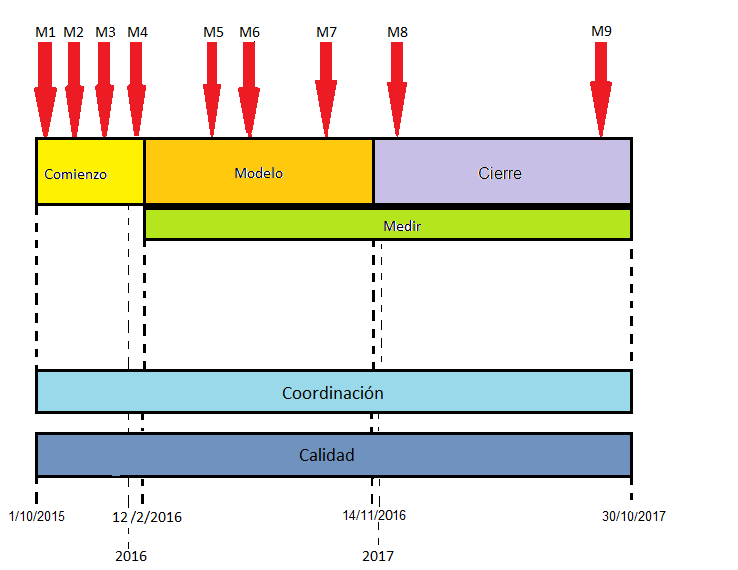
\includegraphics[scale=0.9]{Diagrama_de_Fases.png}
\caption{Localización temporal de cada hito según las fases del proyecto}
\label{fig:Hitos}
\end{center}
\end{figure}

\subsection{Paquetes de trabajo}

El proyecto se va a repartir en doce paquetes de trabajo. La finalidad de cada paquete queda registrada en dos cuadros con las palabras “Título Work Package” y “Objetivos”, seguidos de una explicación más detallada, por pasos, de cómo se llevará a cabo dicho paquete de trabajo, con el título “Descripción de Trabajo”.

Todos los Work Packages (WP), salvo el WP1, tienen además una última sección llamada “Entregables”, en la que se dice lo que se debe presentar para corroborar que el paquete funciona correctamente.

Estos son los paquetes:

\clearpage
\begin{itemize}
\item \textbf{WP1}

\begin{figure}[H]
\begin{center}
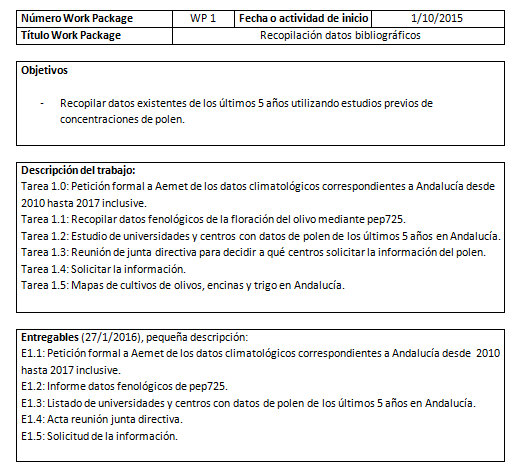
\includegraphics[scale=1]{WP1.png}
\caption{Descripción WP1.}
\label{fig:WP1}
\end{center}
\end{figure}
\clearpage

\item \textbf{WP2}

\begin{figure}[H]
\begin{center}
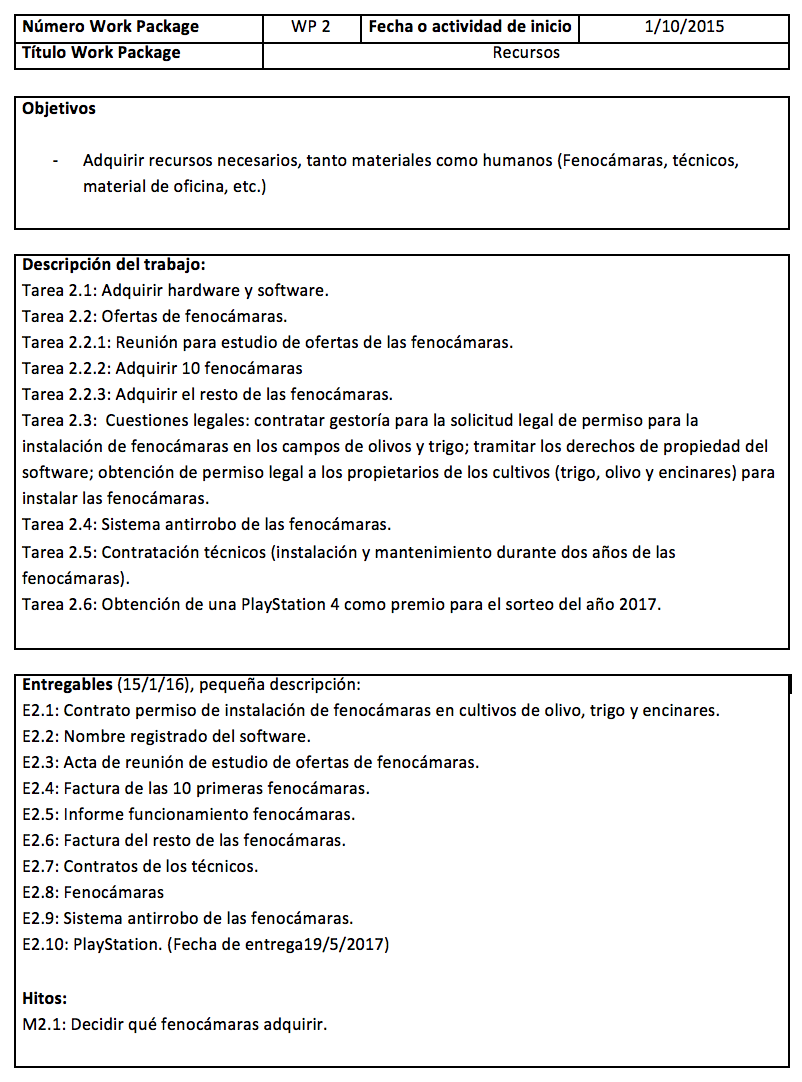
\includegraphics[scale=1.1]{WP2.png}
\caption{Descripción WP2.}
\label{fig:WP2}
\end{center}
\end{figure}
\clearpage

\item \textbf{WP3}

\begin{figure}[H]
\begin{center}
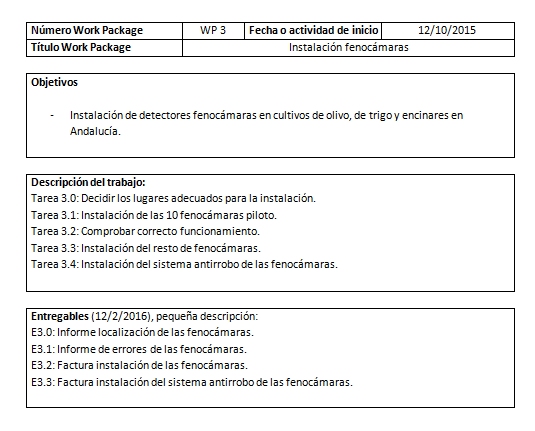
\includegraphics[scale=1]{WP3.png}
\caption{Descripción WP3.}
\label{fig:WP3}
\end{center}
\end{figure}
\clearpage

\item \textbf{WP4}

\begin{figure}[H]
\begin{center}
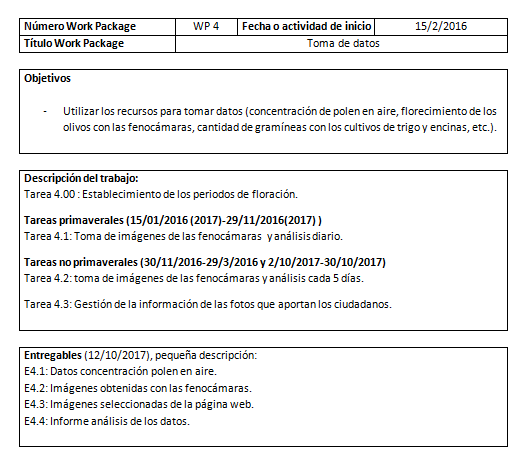
\includegraphics[scale=1]{WP4.png}
\caption{Descripción WP4.}
\label{fig:WP4}
\end{center}
\end{figure}
\clearpage

\item \textbf{WP5}

\begin{figure}[H]
\begin{center}
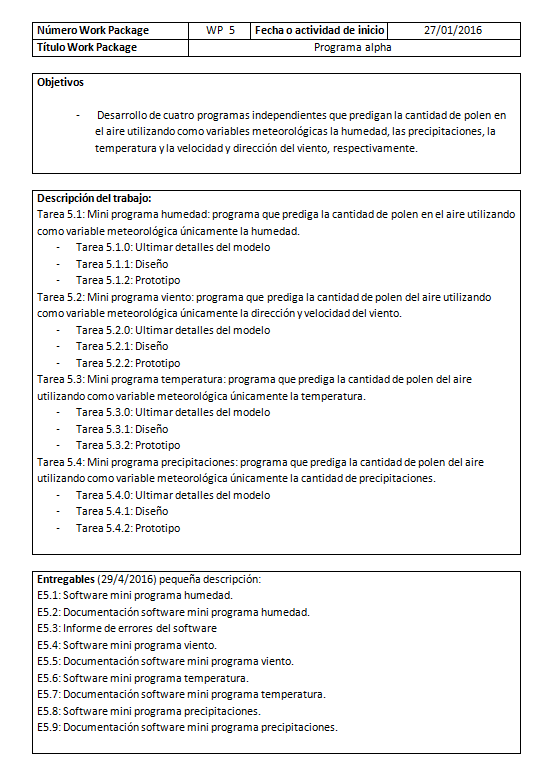
\includegraphics[scale=0.8]{WP5.png}
\caption{Descripción WP5.}
\label{fig:WP5}
\end{center}
\end{figure}
\clearpage

\item \textbf{WP6}

\begin{figure}[H]
\begin{center}
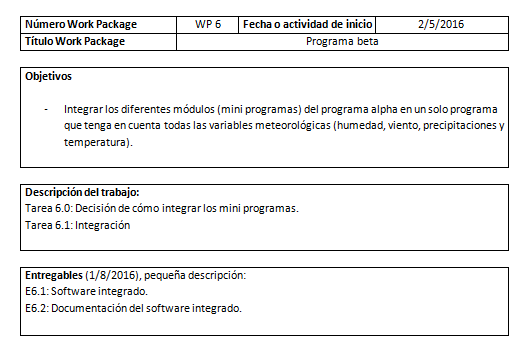
\includegraphics[scale=1]{WP6.png}
\caption{Descripción WP6.}
\label{fig:WP6}
\end{center}
\end{figure}
\clearpage

\item \textbf{WP7}

\begin{figure}[H]
\begin{center}
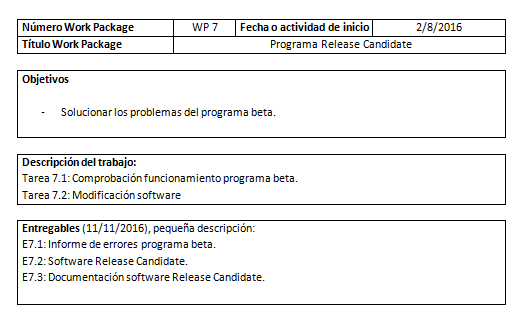
\includegraphics[scale=1]{WP7.png}
\caption{Descripción WP7.}
\label{fig:WP7}
\end{center}
\end{figure}
\clearpage

\item \textbf{WP8}

\begin{figure}[H]
\begin{center}
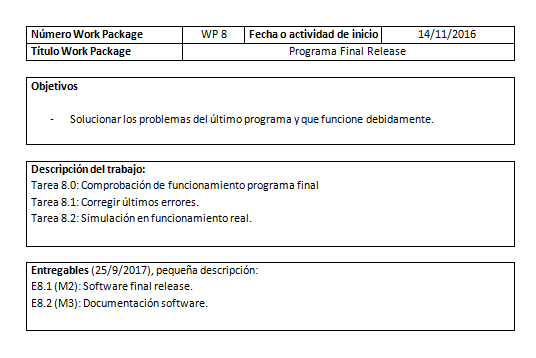
\includegraphics[scale=1]{WP8.png}
\caption{Descripción WP8.}
\label{fig:WP8}
\end{center}
\end{figure}
\clearpage

\item \textbf{WP9}

\begin{figure}[H]
\begin{center}
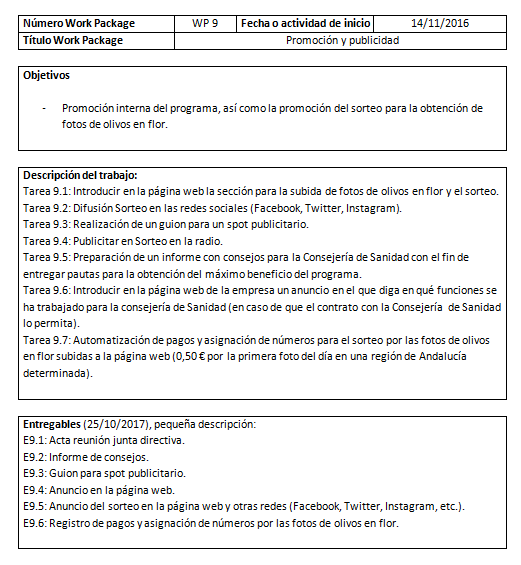
\includegraphics[scale=1]{WP9.png}
\caption{Descripción WP9.}
\label{fig:WP9}
\end{center}
\end{figure}
\clearpage

\item \textbf{WP10}

\begin{figure}[H]
\begin{center}
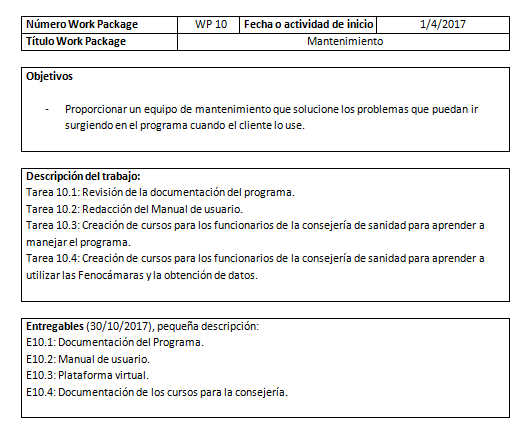
\includegraphics[scale=1]{WP10.png}
\caption{Descripción WP10.}
\label{fig:WP10}
\end{center}
\end{figure}
\clearpage

\item \textbf{WP11}

\begin{figure}[H]
\begin{center}
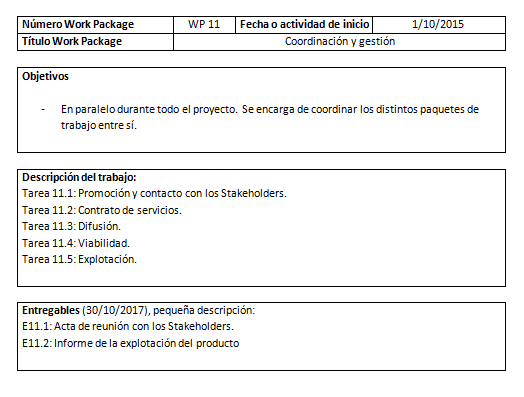
\includegraphics[scale=1]{WP11.png}
\caption{Descripción WP11.}
\label{fig:WP11}
\end{center}
\end{figure}
\clearpage

\item \textbf{WP12}

\begin{figure}[H]
\begin{center}
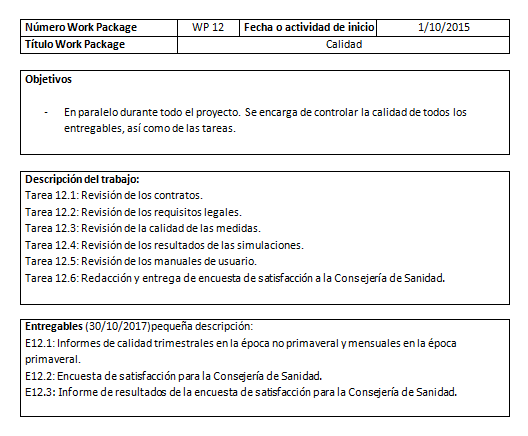
\includegraphics[scale=1]{WP12.png}
\caption{Descripción WP12.}
\label{fig:WP12}
\end{center}
\end{figure}
\end{itemize}
\clearpage


\subsection{Diagrama de Gantt}

El período de cada uno de los WP y las tareas, se describe a continuación de forma gráfica en un Diagrama de Gantt. Es relativamente complejo de entender, de modo que se repartirá en diferentes figuras con explicación. Algunos diagramas se han dispuesto de forma vertical para facilitar la lectura.

La primera figura es básicamente una enumeración de los doce WP, con diferentes datos (detalles al pie de Figura):

\begin{figure}[H]
\begin{center}
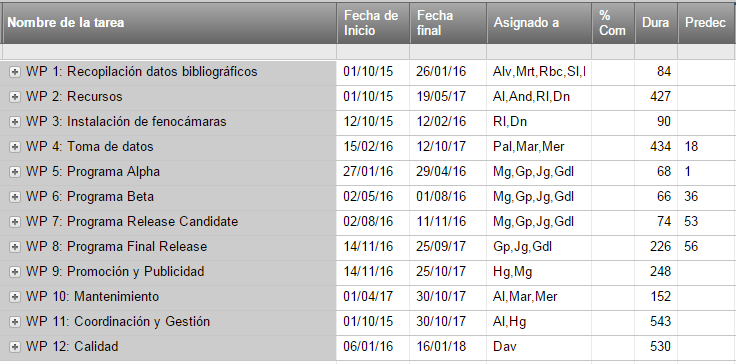
\includegraphics[scale=.8]{Gant1.png}
\caption{Nombre de cada WP, duración en días (con fecha de inicio y de finalización), el responsable de cada tarea, el porcentaje de realización y los predecesores que tiene.}
\label{fig:Gantt1}
\end{center}
\end{figure}

La Figura \ref{fig:Gantt2} es el propio diagrama de Gantt. Para entenderlo hace falta conocer la Figura \ref{fig:Gantt1}. Se pueden imaginar como una única figura alargada partida por la mitad, por motivos obvios de espacio:

\begin{figure}[H]
\begin{center}
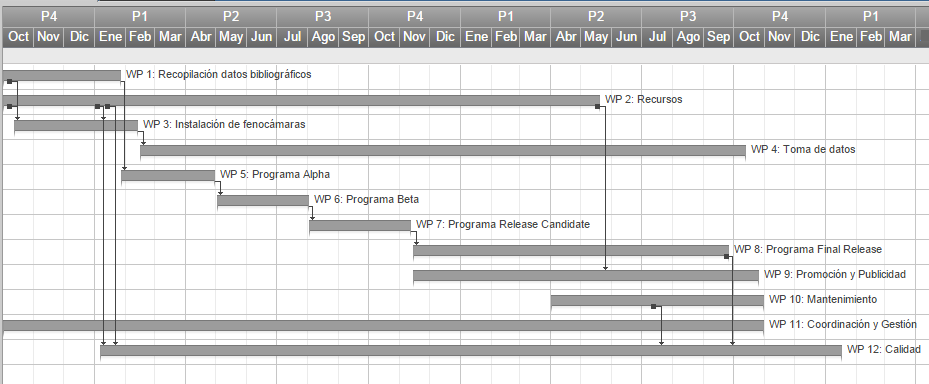
\includegraphics[scale=.7]{Gant2.png}
\caption{Diagrama de Gantt de los WP de la Figura 1. Se ve cómo el proyecto empieza el 1 de octubre del 2015 y termina el 30 octubre de 2017, por lo que el proyecto dura 2 años y un mes.}
\label{fig:Gantt2}
\end{center}
\end{figure}

Por último, las siguientes figuras consisten en doce pequeños diagramas de Gantt, uno para cada Work Package. Las líneas de cada “subdiagrama” pasan a estar en color verde, para diferenciarlas de las grises del Diagrama de Gantt. En orden: WP1-3, WP4-7, WP8-12.

\begin{figure}[H]
\begin{center}
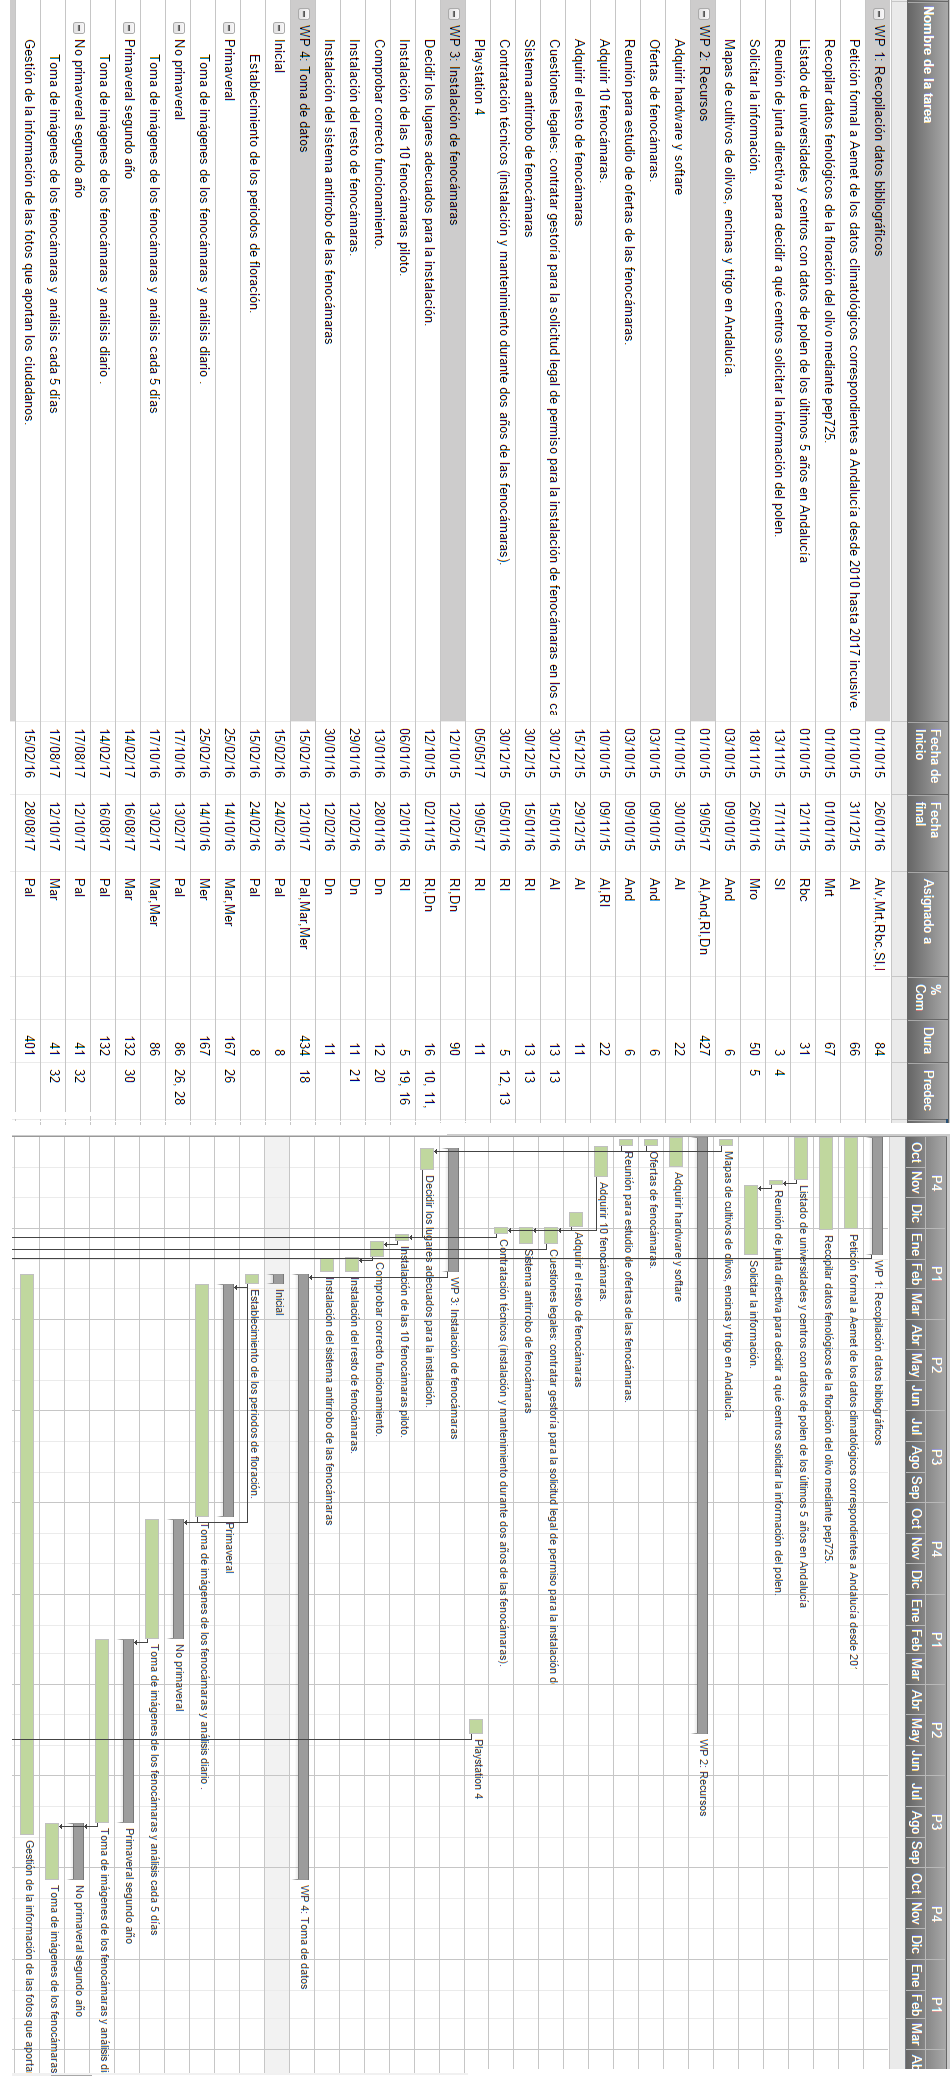
\includegraphics[scale=.45]{Gant3.png}
\end{center}
\end{figure}

\begin{figure}[H]
\begin{center}
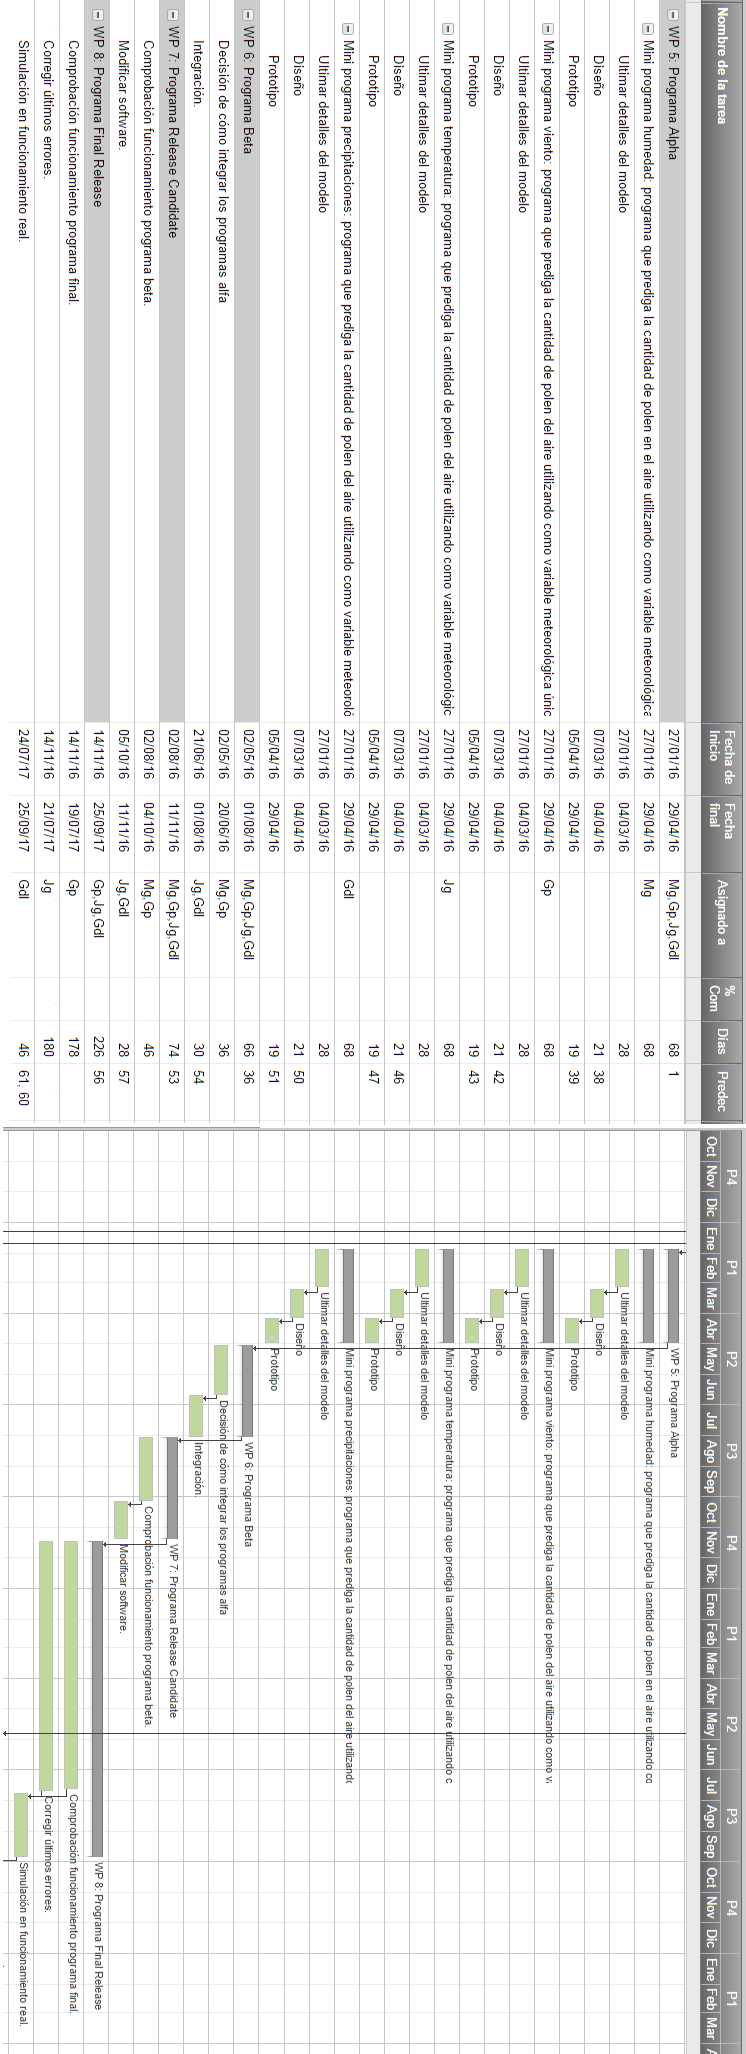
\includegraphics[scale=.45]{Gant4.png}
\end{center}
\end{figure}

\begin{figure}[H]
\begin{center}
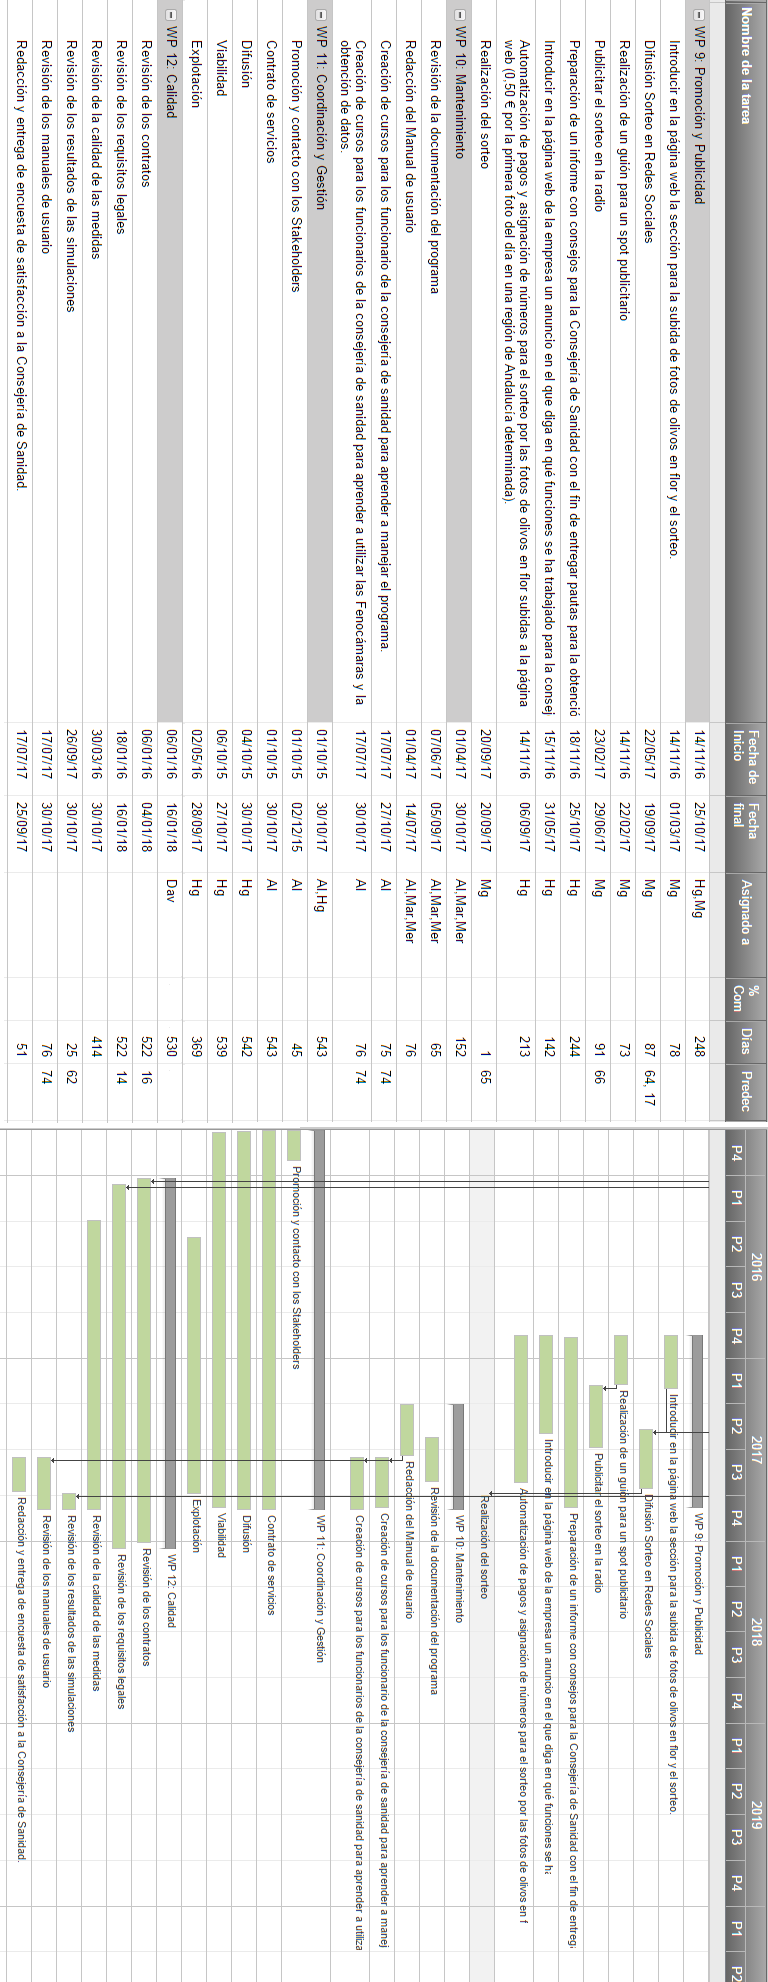
\includegraphics[scale=.45]{Gant5.png}
\end{center}
\end{figure}
\clearpage

\subsection{Hitos}

En la siguiente tabla se recogen los hitos del proyecto.

\begin{figure}[H]
\begin{center}
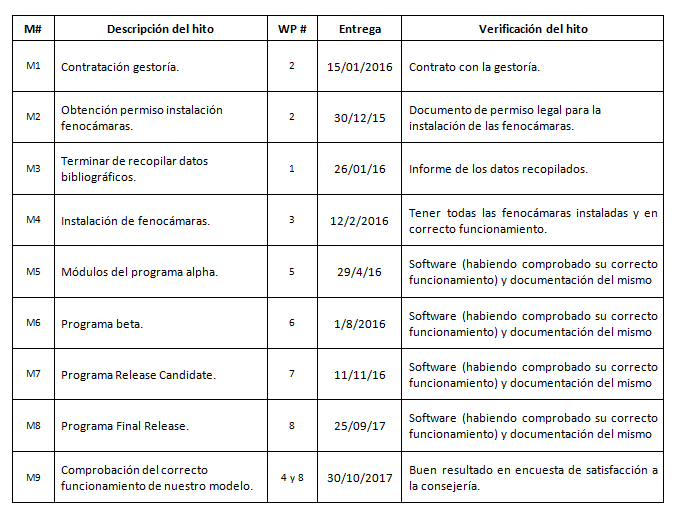
\includegraphics[scale=0.7]{hitos.png}
\end{center}
\end{figure}
\clearpage

\subsection{Entregables}

En las siguientes tablas se recogen los entregables del proyecto.

\begin{figure}[H]
\begin{center}
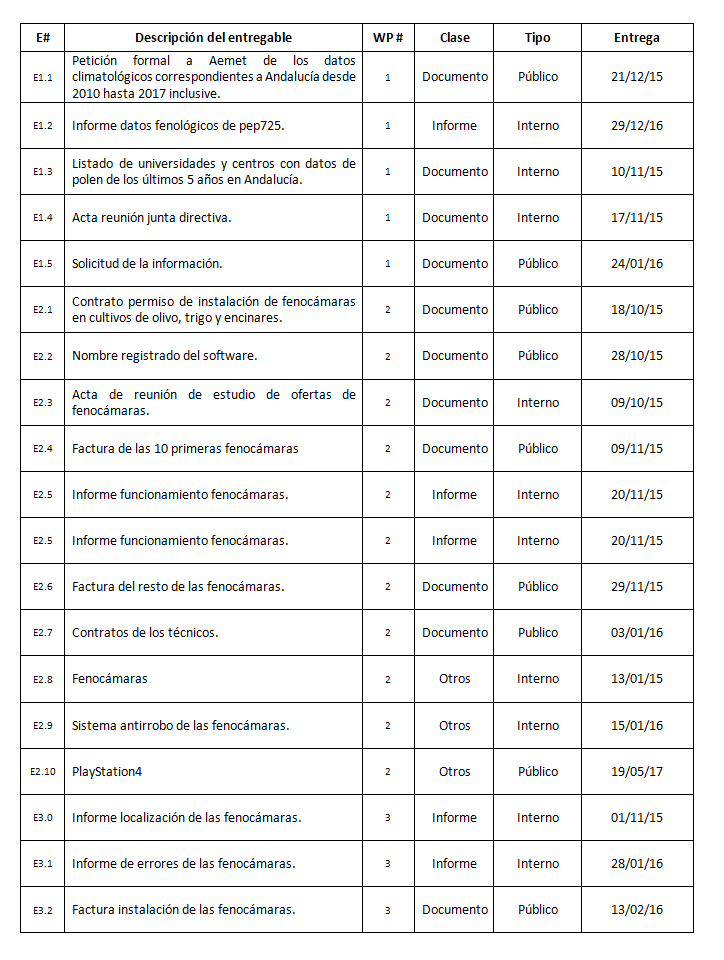
\includegraphics[scale=0.8]{Entregablesp1.png}
\end{center}
\end{figure}

\begin{figure}[H]
\begin{center}
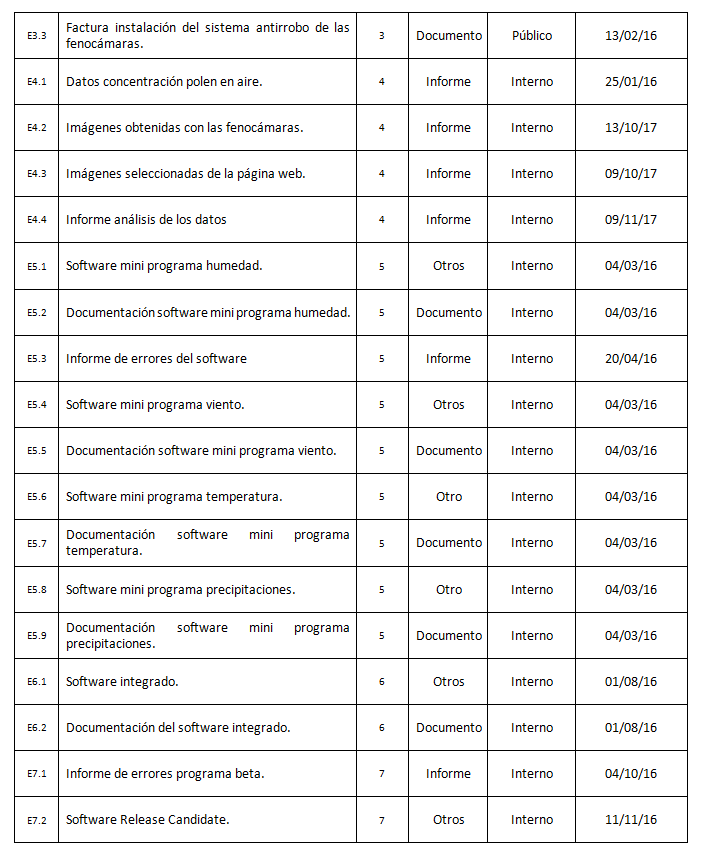
\includegraphics[scale=0.8]{Entregablesp2.png}
\end{center}
\end{figure}

\begin{figure}[H]
\begin{center}
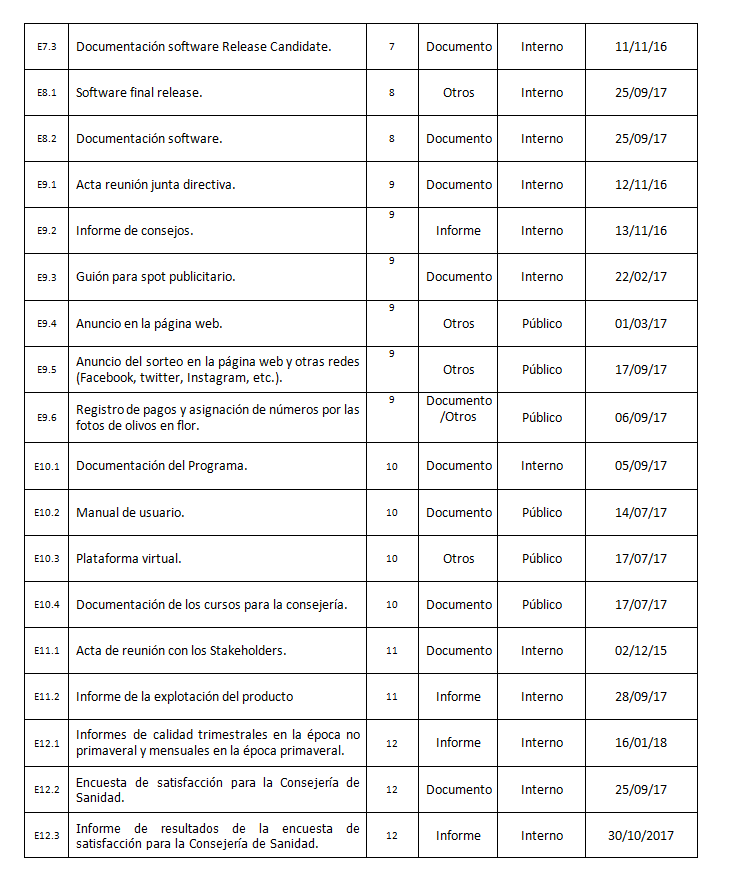
\includegraphics[scale=0.8]{Entregablesp3.png}
\end{center}
\end{figure}
\clearpage

\subsection{Riesgos y contingencias}

Para que la realización de este proyecto se produzca de forma fiable se deben tener en cuenta una serie de riesgos que podrían obstaculizar su desarrollo y disponer de contingencias para amortigüar sus efectos:

\begin{figure}[H]
\begin{center}
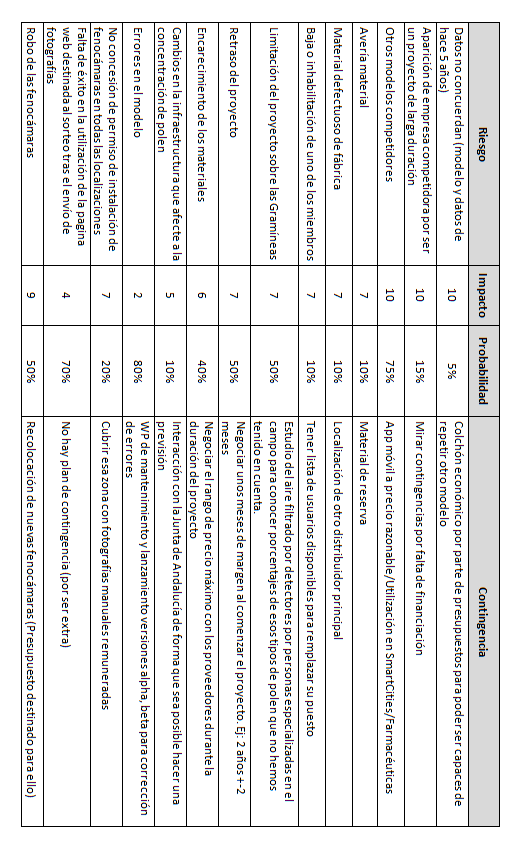
\includegraphics[scale=.8]{RiesgosContingencias.png}
\caption{Lista de los posibles riesgos críticos frente a los que no son críticos para la correcta finalización del proyecto, pero que hay que tener en cuenta.}
\label{fig:Riesgos y Contingencias}
\end{center}
\end{figure}
\clearpage

\subsection{Análisis de stakeholders}

Finalmente, se ha realizado un análisis de los posibles stakeholders: asociaciones, empresas o colectivos interesados en invertir en el proyecto o que están afectados por el mismo.

\begin{figure}[H]
\begin{center}
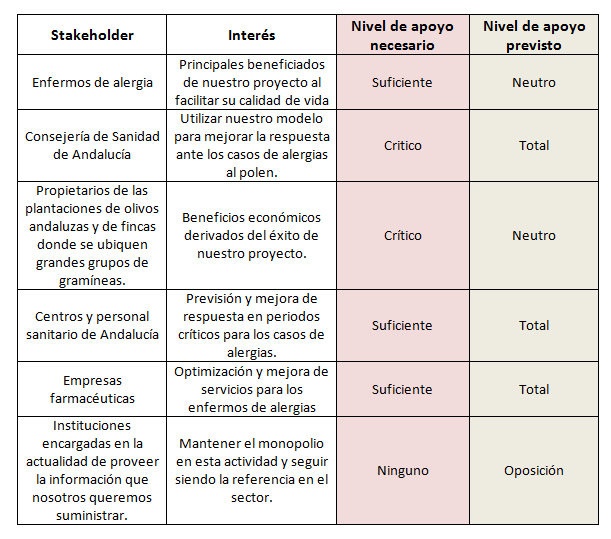
\includegraphics[scale=.7]{stakeholders.png}
\caption{Análisis de stakeholders.}
\label{fig:stakeholders}
\end{center}
\end{figure}
\clearpage



\section{Presupuesto}

Para conseguir llevar a cabo el proyecto presentado, se dispone de un presupuesto que alcanza la cuantía de 1.250.000 Euros y que será distribuido en líneas generales de la siguiente manera:

\begin{figure}[H]
\begin{center}
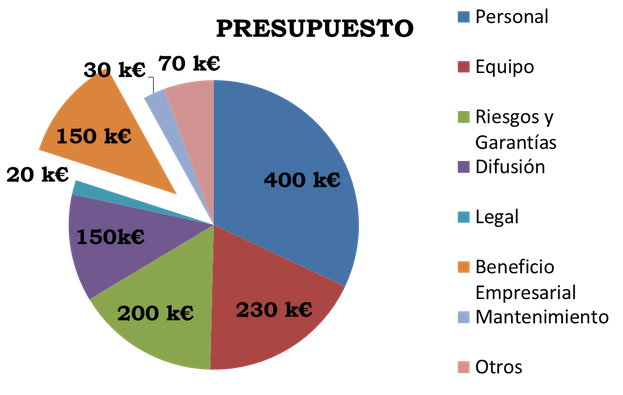
\includegraphics[scale=.9]{Presupuesto.png}
\caption{Definición en términos monetarios del presupuesto empleado en el proyecto.}
\label{fig:Pres1}
\end{center}
\end{figure}

\subsection{Personal}

Se realiza un estimación de las gestiones descritas anteriormente en la sección de planificación, en un total de 40 horas de trabajo efectivo a desempeñar semanalmente en la empresa, con los medios aportados por la misma y en horario a convenir entre las partes, otorgando a cada uno de los trabajadores un mes de vacaciones.

\begin{figure}[H]
\begin{center}
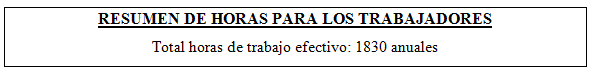
\includegraphics[scale=.8]{Presupuesto2.png}
\end{center}
\end{figure}

(Nota: en caso de que en la realización del trabajo descrito no se llegue a consumir la totalidad de las horas previstas por la ejecución de los trabajos, podrán ser utilizadas para otros servicios que la empresa considere oportunos, siempre que entren dentro del ámbito de actividad del grupo)

En cuanto al personal que se verá implicado directamente en la ejecución del proyecto, se ha clasificado según los honorarios adquiridos acordes a su cualificación y responsabilidad siguiendo 'El Convenio TIC de Salarios':

\begin{itemize}\item Director de proyecto: el hecho de tener más responsabilidad que un Ejecutivo, hace que se le añada un incentivo de 300€ netos al mes en su salario.
\item Técnico Ejecutivo (Ejecutivo): son los responsables de cada uno de los grupos de trabajo: un gerente, un jefe de software, un jefe de coordinación, etc. Forman la cúpula directiva y además de sus correspondientes tareas en sus propios grupos de trabajo, tienen un extra de trabajo y responsabilidad, por lo que son remunerados con 500€ netos al mes, al igual que un Técnico de Alta cualificación.
\item Técnico Especialista (TE): profesionales con estudios universitarios de grado superior (licenciados o máster): programadores, secretarios o administrativos cualificados.
\item Técnico General (TG): profesionales con un grado de cualificación de Diplomatura o Grado.
\item Auxiliar: cualificación de FP: obreros, operarios, auxiliares administrativos, programadores, etc.
\end{itemize}

En la tabla que se muestra a continuación, se recogen los salarios brutos según la cualificación y responsabilidades del personal:

\begin{figure}[H]
\begin{center}
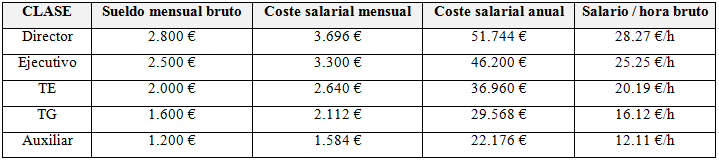
\includegraphics[scale=.8]{Presupuesto3.png}
\caption{Salarios brutos según la cualificación y responsabilidades del personal.}
\end{center}
\end{figure}

(Nota: se ha estimado que las retenciones del sueldo base en IRPF y seguridad social son entorno al 32$\%$, en términos generales)

Cada empleado trabaja en la empresa con unos honorarios acordados con ésta, según la tabla que se acaba de mostrar. Sin embargo no todo su salario procede de este proyecto sino de su trabajo en diferentes tareas dentro de la empresa, por lo que a los trabajadores les corresponderá una parte del presupuesto total del proyecto \textit{'Alergia y polen'}, que será proporcional al número de horas invertidas en la tarea en cuestión. El hecho de que no todo el personal trabaja el mismo número de horas, se cuantifica asignando responsabilidades a cada trabajador, tal como se verá a continuación:

\begin{figure}[H]
\begin{center}
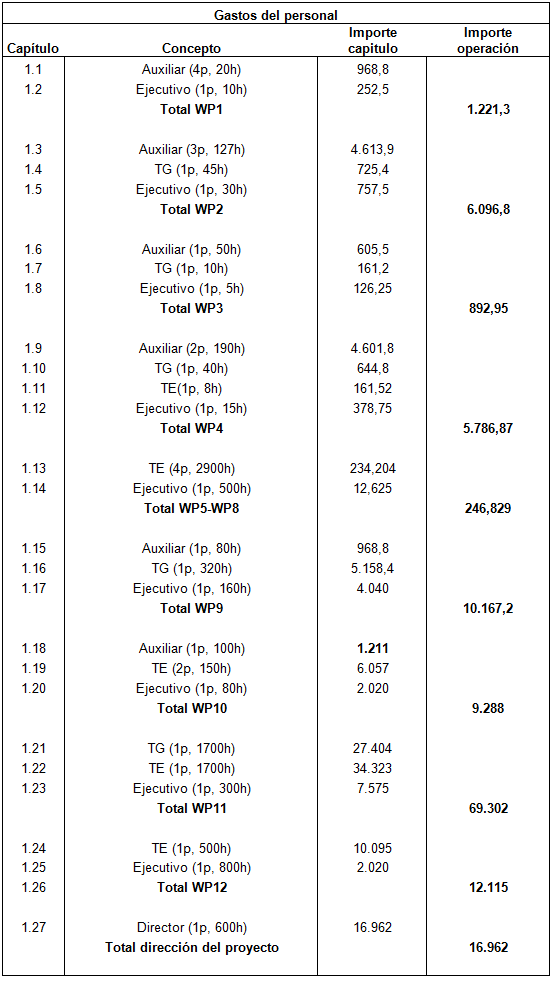
\includegraphics[scale=.8]{Presupuesto4.png}
\caption{Salario de cada trabajador según las características del trabajo desempeñado.}
\end{center}
\end{figure}

Cabe destacar que el número total de los empleados que participan en el proyecto no es un número realista, ya que a lo largo de la ejecución del mismo, algunas personas trabajarán en varios WP diferentes, pudiendo hacer el mismo trabajo la mitad de empleados. Este indicador sirve para estimar la proporción de clases que ha de haber en el proyecto. Asimismo, aunque en la Tabla anterior se recoge un total de 36 empleados, por razones ya mencionadas, para la realización del trabajo se necesitarán 18 empleados según su cualificación:

\begin{figure}[H]
\begin{center}
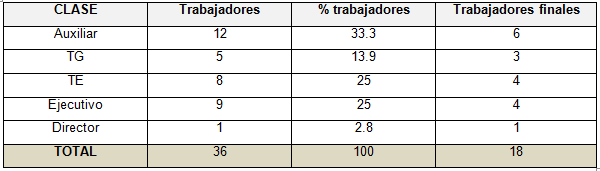
\includegraphics[scale=.8]{Presupuesto_5.png}
\caption{Tabla que recoge los distintos tipos de empleados según su cualificación.}
\end{center}
\end{figure}

\begin{figure}[H]
\begin{center}
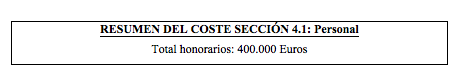
\includegraphics[scale=.9]{Presupuesto6.png}
\end{center}
\end{figure}

El importe total aquí indicado está calculado en función del tiempo estimado según los antecedentes manifestados por la empresa y podrán ser objeto de revisión en función de las horas incurridas efectivas para el desarrollo de los trabajos encargados. Asimismo, observando el coste total en horas de los honorarios, podemos estimar que el porcentaje del presupuesto total destinado a personal será del 32$\%$.


\subsection{Equipo}

En cuanto al equipo necesario para la ejecución del proyecto, se tendrán en cuenta aquellos que sólo sean genuinos al mismo. Se define además, que cada trabajador dispone de una mesa, silla y ordenador de proyectos anteriores, por lo que dichos gastos no entran dentro del proyecto. 

A continuación se muestra el inventario empleado para la ejecución del proyecto que supone un coste.

\subsubsection{Cámara con módulo 3G}

Cámara IP tamaño mini: emite imágenes directamente a la red, intranet o internet, sin necesidad de ordenador.

En un primer momento se realizó una estimación a grosso modo, en la cual se requerían 5 cámaras IP tamaño mini por municipio para controlar las plantaciones de olivo, lo cual llevaba a la instalación de unas 3100 cámaras para los 774 municipios que conforman la comunidad andaluza. Además, también se usarían este tipo de cámaras para monitorizar grandes extensiones de cultivo de trigo y encinas, con lo que el número ascendía a una cuantía de 5000 cámaras, algo totalmente inviable para la realización del proyecto. Por dicha razón se ha realizado un estudio exhaustivo desde el departamento de presupuestos, para optimizar los recursos necesarios para llevar a cabo el proyecto. (Apéndice I: Estudio de la optimización de recursos). A partir de la realización de dicho estudio se emplearán un total de 1700 cámaras para cubrir las plantaciones de interés:

\begin{figure}[H]
\begin{center}
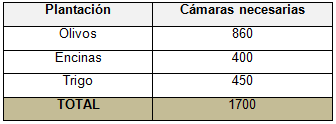
\includegraphics[scale=.8]{Presupuesto7.png}
\caption{Estimación de cámaras necesarias para los distintos tipos de plantaciones.}
\end{center}
\end{figure}

\subsubsection{Software de reconocimiento de imágenes: ADCIS}

Cuenta con una amplia gama de funciones para el tratamiento y análisis de imágenes, una gran variedad en cuanto a los tipos de medidas, una serie de herramientas de dibujo que permiten extraer rápidamente medidas cuando la segmentación se revela con dificultad, y una inmensa lista de posibilidades avanzadas gracias a módulos opcionales.

En la Tabla que se muestra a continuación, se recogen los costes asociados a las herramientas que conforman el inventario, y que serán utilizadas para la realización del proyecto:

\begin{figure}[H]
\begin{center}
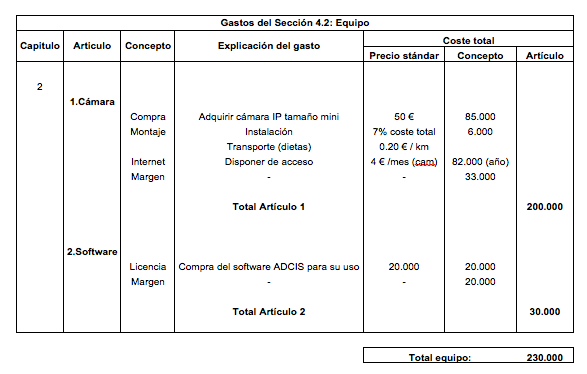
\includegraphics[scale=.8]{Presupuesto8.png}
\caption{Costes del equipo necesario para la realización del proyecto.}
\end{center}
\end{figure}

Tal como se ha podido comprobar, la sección presente conforma los materiales y herramientas necesarias para la realización del proyecto, parte que dispone una cuantía de 230.000 Euros, que representa el 18.4 $\%$ del presupuesto total.

\begin{figure}[H]
\begin{center}
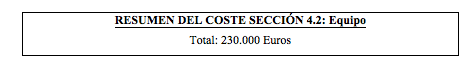
\includegraphics[scale=.9]{Presupuesto9.png}
\end{center}
\end{figure}


\subsection{Riesgos y garantías}

Esta categoría engloba dos importantes secciones:

\begin{itemize}
\item Riesgos: se tienen en cuenta los diferentes riesgos, su impacto y el coste económico asociado a los mismos y a los planes de contingencia.
\item Garantías: incluye cualquier tipo de error, rotura o imprevisto que la empresa se compromete a subsanar sin coste adicional del cliente. Son averías en las cámaras, fallos en el software, errores en la toma de datos, etc.
\end{itemize}


\subsubsection{Riesgos}

En este artículo es donde se tienen en cuenta diferentes acciones que pueden poner en peligro al proyecto, el impacto que pueden ocasionar y el coste económico asociado a las mismas y a los planes de contingencia ya trazados.

Es evidente, que aquellos riesgos que tienen un mayor impacto son aquellos que hagan que el proyecto se retrase, ya que cuánto más tiempo se necesite para realizar tareas con  plazos marcados de ante mano mayor coste en sueldos y equipamiento serán necesarios para la ejecución de una misma tarea.

Un segundo factor de riesgo por el que puede verse amenazado el proyecto es la estafa, el robo y/o el encarecimiento de los materiales y algunas herramientas empleadas. Por todo lo demás, la empresa queda exenta, ya que los gastos están cubiertos: los costes en material y herramientas defectuosas o averías se encuentran en garantías, y son cubiertos de fábrica.

Para cubrir estos riesgos, sin poner en ningún momento en peligro al proyecto y la continuidad del mismo, se destinará un porcentaje del presupuesto total para hacer frente a los riesgos asociados a la pérdida de las cámaras, bien sea para cubrir su posible ruptura y/o robo, el cableado, o nuevas instalaciones. Además, se reserva una cuantía del presupuesto en caso de que, por motivos ajenos, bien sea una enfermedad o una baja médica, se necesite contratar personal cualificado (sustitución).

(Nota: destacar que las cámaras serán instaladas en plantaciones de olivos, encinas y trigo, con lo que se contempla que éstas poseen ya sus propios sistemas antirrobo, bien tradicionales o modernos, para la preservación de sus propios productos. Así pues, esta protección es aplicada indirectamente a la cámaras instaladas, por lo que el riesgo de robo queda reducido, más allá de nuestras propias medidas disuasorias)


\subsubsection{Garantías}

En este punto es donde las empresas con las que se cuenta para la realización del proyecto se comprometen con el cliente (nosotros), sin coste alguno, a subsanar cualquier tipo de error, rotura y/o imprevisto tales como averías en las cámaras, fallos en el software, errores en la toma de datos, etc.

Dado que en la sección 4.3.1 Riesgos, se ha reservado ya una cantidad de dinero en caso de que fuera necesario comprar cámaras. En la sección 4.3.2 que aquí se trata, se ha estimado que al menos, todas las cámaras que disponemos se rompan  1.15 veces, por lo que se le añadirá un 15$\%$ adicional del presupuesto en dicho concepto.

No obstante, debe tenerse en cuenta además los honorarios del personal que trabajará en atención al cliente, como en los servicios de mantenimiento-reparaciones, por lo que se destinará cierta cuantía para dicho fin. En la Tabla que se muestra a continuación se recoge el coste asociado a la sección 4.3, desglosado en cada uno de los artículos aquí explicados:

\begin{figure}[H]
\begin{center}
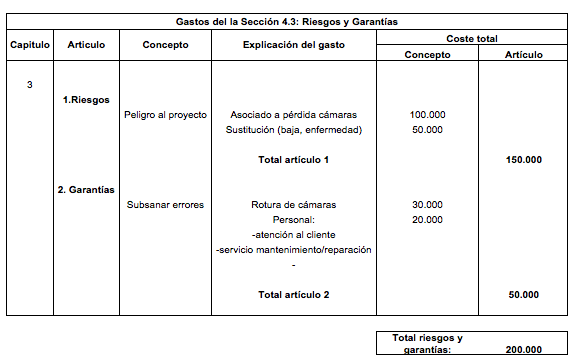
\includegraphics[scale=.8]{Garantias.png}
\end{center}
\end{figure}

Tal como se ha podido comprobar, la sección 4.3 que conforma los riesgos y garantías a los que se encuentra expuesto el proyecto, dispone de una cuantía que asciende a los 200.000 Euros, que representan el 16$\%$ del presupuesto total.

\begin{figure}[H]
\begin{center}
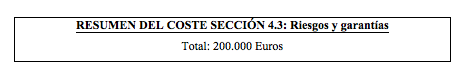
\includegraphics[scale=.8]{Garantias2.png}
\end{center}
\end{figure}


\subsection{Marco legal}

Atendiendo a las necesidades jurídicas y aspectos legales, una parte del presupuesto irá destinada a ello, a través de la contratación de una gestoría para promover, solicitar y realizar toda clase de trámites, solicitudes o cualquier función de ámbito administrativo, informando del estado y vicisitudes del procedimiento que se lleva a cabo a la empresa, para que esté al tanto de todo.

Además, se realizará un registro de la propiedad intelectual del resultado del proyecto realizado, siendo dicho registro un mecanismo administrativo para la protección de los derechos de propiedad intelectual de los autores y demás titulares que han participado en este trabajo. Así mismo, la inscripción registral, supone una protección de los derechos de propiedad intelectual, en tanto que constituye una prueba cualificada de la existencia de los derechos inscritos. Cabe mencionar, que también se realizará un registro de la marca, patentes y licencias derivadas de dicho proyecto.

\begin{figure}[H]
\begin{center}
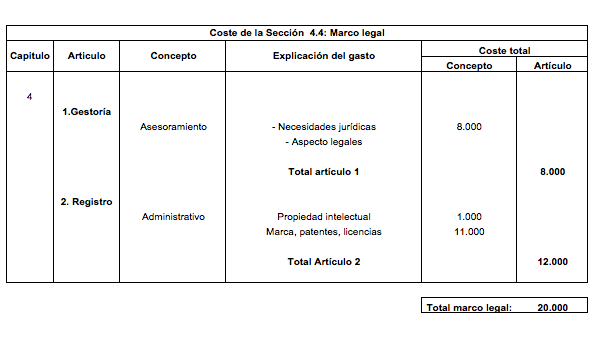
\includegraphics[scale=.8]{Legal.png}
\caption{Presupuesto destinado a los distintos aspectos del marco legal del proyecto.}
\end{center}
\end{figure}

Tal como se puede ver en la tabla anterior, el Capítulo 4: Marco legal, dispondrá de la cuantía de 20.000 Euros, que corresponde al 1.6$\%$ del presupuesto total destinado al proyecto.

\begin{figure}[H]
\begin{center}
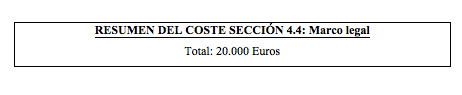
\includegraphics[scale=.8]{Legal2.png}
\end{center}
\end{figure}


\subsection{Difusión}

Dicha sección tiene un gasto considerable incluido en los honorarios de los participantes del proyecto, los cuales están incluidos en la sección 4.1 Personal. No obstante, se destinará cierta cantidad del presupuesto para el gasto en materiales, promoción interna, diseño de una página web, y en marketing donde se incluye la publicidad y la difusión externa. 

Referente a la publicidad y difusión externa, se utilizarán como medio de comunicación periódicos y radios locales y/o regionales. Concretamente, se pretende transmitir la puesta en marcha de la iniciativa “Fotografía floral”, en la que se incentiva la participación de los ciudadanos para la monitorización de la floración de los olivos, encinas y cultivos de trigo. Además, se realizarán una serie de eventos en locales o centros de investigación y/o enseñanza para dar a conocer la propuesta y el proyecto. No obstante, todo lo aquí mencionado se recoge más detalladamente en el Apéndice II: Difusión.

\begin{figure}[H]
\begin{center}
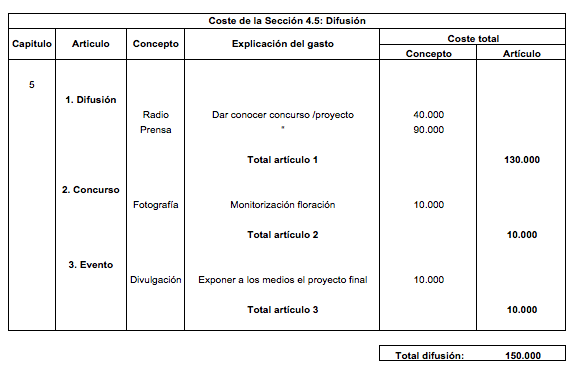
\includegraphics[scale=.8]{Difusion.png}
\end{center}
\end{figure}

Tal como se muestra en la tabla anterior, el Capítulo 5: Difusión, dispondrá de la cuantía total de 150.000 Euros, que corresponde con el 12$\%$ del presupuesto total destinado al proyecto.

\begin{figure}[H]
\begin{center}
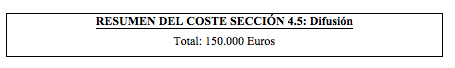
\includegraphics[scale=.8]{Difusion2.png}
\end{center}
\end{figure}

\subsection{Mantenimiento}

Tras la finalización del proyecto, la empresa habrá sido capaz de desarrollar una herramienta que se pondrá en el mercado. Asimismo, el mantenimiento de la misma será llevado a cabo por el cliente una vez cerrado el proyecto, por lo que la empresa debe asegurar un modo de cubrir el servicio sin hacerse cargo directamente.

Como una manera de salvaguardar dicha herramienta, se formarán a personas con diferentes perfiles académicos que cumplan una serie de requisitos con el objetivo de transmitir los conocimientos técnicos necesarios para manejar la herramienta, así como cuidar las cámaras ,el software y demás. 

Los cursos ofertados se centrarán en el mantenimiento y funcionamiento del producto final del proyecto. Éstos serán ofrecidos entre 3 y 6 veces al año durante los 4 años consecutivos a la clausura del proyecto. Además, serán jornadas intensivas de 6 horas durante 3 días, impartidas por un profesor experto en el tema (categoría TE).

Para dicho fin, la sección 4.6: Mantenimiento, contará con una cuantía de 30.000 euros en concepto de cursos de formación, lo cual representa el 2.4$\%$ del presupuesto total disponible.

\begin{figure}[H]
\begin{center}
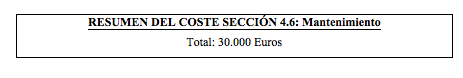
\includegraphics[scale=.8]{Mantenimiento.png}
\end{center}
\end{figure}


\subsection{Beneficios empresariales}

Esta sección recoge el beneficio empresarial por la realización del proyecto, que aquí se está presentando. Por ello, se ha realizado una estimación y la empresa con la realización de dicho proyecto ganaría una cuantía que asciende a los 150.000 euros, lo que supone un 12$\%$ del presupuesto total del proyecto.

(Nota: en caso de necesitar capital para afrontar la sección 4.3. Riesgos y Garantías, se tomará de es capítulo aquí tratado la cantidad necesaria)

\begin{figure}[H]
\begin{center}
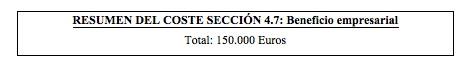
\includegraphics[scale=.8]{Beneficios.png}
\end{center}
\end{figure}


\subsection{Otros}

Dicho capítulo ha sido creado, para justificar el capital sobrante que en primera estancia no está previsto utilizar, pero que está disponible en casos como los que se verán a continuación:

\begin{figure}[H]
\begin{center}
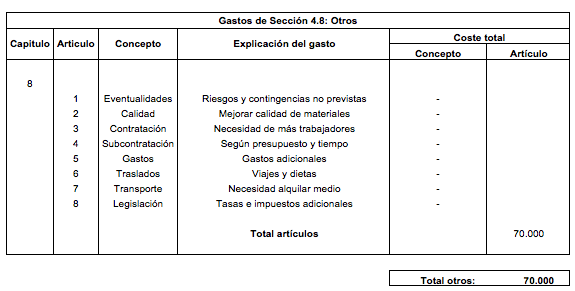
\includegraphics[scale=.8]{Otros.png}
\end{center}
\end{figure}

Tal como se ha podido comprobar, cada uno de los artículos que conforman la sección 4.8: Otros, dispone de una cuantía, en su totalidad,  que asciende a los 70.000 Euros, que representan el 5.6$\%$ del presupuesto total.

\subsection{Resumen}

La siguiente tabla presenta un resumen de las asignaciones  de presupuesto a las diferentes partes del proyecto.

\begin{figure}[H]
\begin{center}
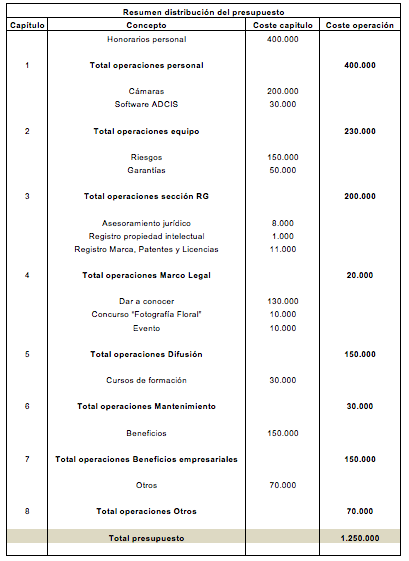
\includegraphics[scale=1]{Presupuesto10.png}
\caption{Resumen de las asignaciones de presupuesto.}
\end{center}
\end{figure}

\clearpage


\section{Apéndice I: Estudio de la optimización de recursos}

Para estimar la fenología de las gramíneas correlacionaremos datos obtenidos de la floración de los olivos, encinas y trigo. Para realizarlo será necesario crear una red de cámaras que nos permita llevar un control exhaustivo de las diferentes plantaciones. Se desecha la opción de utilizar repetidores \textit{m2m} ya que cada aparato cuesta unos 2000 € y se necesitan demasiados para cubrir el extenso área. Por eso utilizaremos servicio internet (3G) que producirá un gasto por uso de cada cámara de en torno a 4 €/mes.

En primer lugar se muestra la distribución de olivos en toda la comunidad de Andalucía:

\begin{figure}[H]
\begin{center}
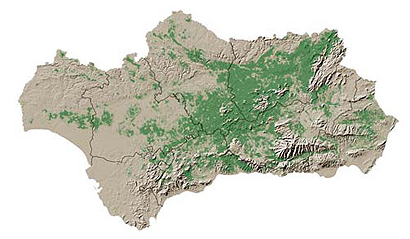
\includegraphics[scale=.9]{Apendice1.png}
\caption{Resaltado en verde se representa la distribución de las plantaciones de olivos por la Comunidad Autónoma de Andalucía.}
\end{center}
\end{figure}

Tal como se puede ver, las plantaciones de olivares cubren mayoritariamente las provincias de Jaén y Córdoba, y en menor medida las de Málaga, Granada y Sevilla. Con el objetivo de determinar el número de cámaras necesarias para cubrir dicha extensión, supondremos que las provincias con mayor número de plantaciones están completamente cubiertas, mientras que el resto de provincias estarán vacías de olivares. De este modo se puede estimar en promedio el área a cubrir para, así, obtener una primera aproximación del número de cámaras necesarias para monitorizar el proceso de floración del olivo en Andalucía.

Se sabe que las provincias de Jaén y Córdoba tienen 97 y 75 municipios respectivamente. Suponiendo que cada uno de los municipios presenta unas características geográficas y climáticas similares en toda su extensión, se obtiene que utilizar 5 cámaras por municipio son suficientes para monitorizar las plantaciones de olivos. Por lo cual, extendiendo este resultado a toda la superficie que debemos analizar, el número de cámaras totales será de 860.

Para la optimización del número de cámaras empleadas para cubrir las plantaciones de encinas y trigo, realizaremos el mismo procedimiento que para los olivos. Para llevar un control sobre los campos de encinas, utilizaremos los grandes pastos para las piaras, de Andalucía. Ésta es la zona mas interesante para situar nuestras cámaras, ya que 
aparte de poseer una gran concentración de encinas, son zonas que se encuentran protegidas por perros y guardeses. Las principales zonas de piara de Andalucía son:

\begin{figure}[H]
\begin{center}
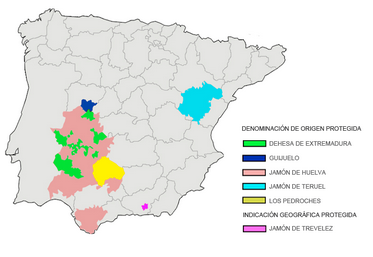
\includegraphics[scale=.9]{Apendice2.png}
\caption{Mapa de la Península Ibérica donde están resaltados con diferentes colores las principales zonas de piara.}
\end{center}
\end{figure}

Utilizando un procedimiento similar al anterior y observando el mapa expuesto, podemos aproximar el área de encinas de Andalucía como la totalidad de la provincia de Huelva. Ésta tiene un total de 80 municipios. Colocando 5 cámaras por municipio obtenemos que será necesario instalar un total 400.

Por último las plantaciones de cereal de secano en Andalucía se encuentran principalmente distribuidas en las provincias de Sevilla y Cádiz.

\begin{figure}[H]
\begin{center}
\includegraphics[scale=.9]{Apendice3.png}
\caption{Mapa de Andalucía donde se ha representado la superficie cubierta por las diferentes plantaciones y cultivos.}
\end{center}
\end{figure}

Como nos vamos a centrar en el trigo, asumiremos pues que la totalidad de la superficie de cereales de secano se refieren al trigo para simplificar el problema.Entre las dos provincias que se han mencionado hacen un total de 150 municipios, y la idea es instalar 3 cámaras por municipio, con lo que se utilizarán para este respecto un total de 450 cámaras.

En términos generales serán necesarias aproximadamente 1700 cámaras.


\section{Apéndice II: Difusión}

Hay que tener en cuenta que el proyecto debe ser difundido para que la gente y posibles \textit{sponsors} lo conozcan. Es más, se va a realizar un concurso de fotografía así que es importante difundirlo de alguna manera. Para ello los medios principales de comunicación que se van a usar son prensa y radio, preferiblemente a nivel regional.

La difusión por prensa consiste en dar a conocer el concurso mediante anuncios y/o artículos que informen sobre las bases y las fechas en las que tendrá lugar. La concentración de olivos, encinas y gramíneas es mayor en las regiones de Jaén, Córdoba, Huelva, Sevilla y Cádiz, por lo que serán esas provincias en las que se difunda principalmente.

En cuanto a la difusión vía radio, se realizarán cuñas de treinta segundos que informen también de las bases del concursos. Del mismo modo, se pretende asistir a tertulias con el objetivo de dar a conocer ya no sólo el concurso sino también el proyecto.

Las bases del concurso aún están por delimitar de forma concreta pero será a grandes rasgos un concurso de fotografía corriente, en el que se busca que la gente salga a la calle y fotografíe olivos y encinas que escapen a nuestras cámaras. Se pagará por cada foto relevante recibida y el ganador recibirá un premio que consistirá en una videoconsola “PlayStation 4”.

Finalmente se pretende organizar una serie de eventos para todos los públicos, desde charlas en locales hasta centros de investigación (especialmente universidades), con el fin de dar a conocer este proyecto.


\section{Apéndice III: Estrategias de empresa}

La siguiente matriz es un análisis SWOT. Representa las diferentes características internas (fortalezas S y debilidades W) y factores externos (oportunidades O y amenazas T) que deben tenerse en cuenta para planificar una estrategia de futuro que tenga en cuenta cambios externos al proyecto. Las posibles estrategias de actuación frente a cada uno de los factores que aparecen en la matriz SWOT se presentan dentro de la propia matriz.

\begin{figure}[H]
\begin{center}
\includegraphics[scale=.7]{SWOT.png}
\caption{Matriz SWOT. (Fortalezas $S$, debilidades $W$, oportunidades $O$ y amenazas $T$)}
\label{fig:SWOT}
\end{center}
\end{figure}

Como estrategias S-O, usando las virtudes de la empresa para aprovechar las oportunidades se tiene:

\begin{itemize}
\item Ofertar a los agricultores que, a cambio del permiso para monitorizar sus cosechas, tengan acceso a la información recopilada y conocimiento sobre el estado actual de su cosecha sin necesidad de estar de forma física en la plantación.
\item Se pueden aprovechar las fotografías de los olivos para garantizar la salud y calidad del cultivo de ese año.
\item El mercado del aceite de oliva es de gran importancia en España. Garantizar que los cultivos tienen calidad, estudio que se puede hacer mediante las fotografías tomadas, puede interesar a muchas empresas del sector.
\end{itemize}

Para minimizar las debilidades internas y potenciar las posibilidades de obtener oportunidades se han diseñado los siguientes planes de acción (estrategias W-O):

\begin{itemize}

\item Debido a la escasa formación en el tema de las alergias al polen por parte del personal de la empresa, el acceso a cursos y la especialización de algunos empleados son un avance importante para solventar el problema.
\item Existen subvenciones por parte de diferentes organismos que financian proyectos que resulten emprendedores.
\end{itemize} 

Aprovechando los puntos fuertes del proyecto contra las amenazas externas se hace uso de la siguiente estrategia (estrategia T-S):

\begin{itemize}
\item Se pueden buscar alianzas entre empresas. Por ejemplo, hacer un trato con INTA (Instituto Nacional de Técnica Aeroespacial), permitiría el uso de satélites y RPAs a menor coste y con ambos dispositivos a nuestra disposición se podrían obtener nuevas imágenes que cubran áreas que las fenocámaras no llegan a cubrir.
\end{itemize}

Debe tenerse un plan que para solventar las amenazas teniendo en cuenta las debilidades del proyecto, por lo que dispone del siguiente plan de acción (estrategia W-T):

\begin{itemize}
\item Debido a la sencillez del modelo, el proyecto puede desarrollarse como un plan piloto a la espera de que se realice un desarrollo más profundo en este campo en los próximos años, teniendo ya una serie de referencias anteriores obtenidas del plan piloto realizado por nuestra empresa.
\end{itemize}



\section{Apéndice IV: Estudio de la posibilidades de expansión del proyecto}

En este apartado se valora la posibilidad de una expansión del proyecto en busca de otras partes interesadas en los datos o resultados que maneja el proyecto. Se ha elaborado la siguiente lista:

\begin{itemize}
\item En primer lugar, los agricultores. Para poder monitorizar las cosechas, ofertar a los agricultores el acceso a la información recopilada y conocimientos sobre el estado de su cosecha sin tener que pagar por ello. Esto les permitirá no tener que desplazarse físicamente hasta la cosecha para comprobar su estado, además de poder llevar un control más detallado de estas.
\item El aprovechamiento de las imágenes podría ayudar también a garantizar la salud y el buen estado del cultivo de ese año, y a realizar una estimación de los posibles beneficios de la cosecha. Estas predicciones podrían resultar de interés tanto a los propios agricultores como a empresas cuyos productos dependan de las mismas (por ejemplo, las empresas de aceite de oliva).
\item Finalmente, el mercado del aceite de oliva en España se ha convertido en el más importante a nivel mundial, a base de mantener un alto grado de producción, y realizar grandes exportaciones a países como China o Estados Unidos. Este mercado reporta gran cantidad de beneficios y es un pilar fundamental de la economía y de la identidad de nuestro país. Sin llegar más lejos, y para hacernos una idea del impacto que tiene en nuestra economía, en el año 2014 Andalucía, el principal productor de aceite, exportó cerca de 848.000 toneladas de aceite de oliva por valor de 2.015 millones de euros. Por lo tanto, el principal objetivo del mercado es incrementar el consumo de aceites de oliva a nivel mundial, mejorando a su vez la imagen de productos de calidad de los aceites de oliva de España. Para continuar creciendo y mejorar la competitividad y sostenibilidad es fundamental promover soluciones y medidas que permitan controlar lo mejor posible la producción anual, minimizando las perdidas.  Para ello, la toma de imágenes realizadas en nuestro proyecto, puede convertirse en una importante fuente de información fiable, tanto para los agricultores como para las empresas distribuidoras, y reportar gran cantidad de beneficios, marcando la diferencia con los distintos competidores del mercado mundial.
\end{itemize}





\section{Apéndice V: Planificación alternativa para 1 año}

Se ha elaborado asimismo un diagrama de Fases con una planificación alternativa en caso de que el proyecto debiera llevarse a cabo solamente en 1 año.

\begin{figure}[H]
\begin{center}
\includegraphics[scale=.6]{Diagrama_GP.png}
\caption{Diagrama  con la planificación del proyecto basada en solamente 1 año.}
\end{center}
\end{figure}


\section{Apéndice VI: Calidad}

Un informe de calidad del proyecto puede ser encontrado adjunto al mismo.


\section{Referencias}

Páginas web visitadas por última vez el 09/03/2015.

\begin{enumerate}

\item \verb|www.uco.es/aerobiologia/fenologia/olivo.html|
\label{ref:uco1}

\item \verb|http://www.uco.es/aerobiologia/fenologia/gramineas.html|
\label{ref:uco2}

\item \verb|http://www.uco.es/aerobiologia/fenologia/quercus.html|
\label{ref:uco3}

\item \verb|http://imagenes.forociudad.com/fotos/209685-valdefuentes-flores-de-encina.jpg|
\label{ref:flor_encina}

\item \verb|http://www.ugr.es/~aerobio/imagenes/calendarioJ.gif|
\label{ref:calen_J}

\item \verb|http://www.ugr.es/~aerobio/imagenes/calendarioA.gif|
\label{ref:calen_A}

\item \verb|http://www.ugr.es/~aerobio/imagenes/calendarioG.gif|
\label{ref:calen_G}

\item \verb|http://www.ub.edu/geocrit/sn/sn-416_archivos/image003.jpg|
\label{ref:especies_andalucia}

\item \verb|http://www.juntadeandalucia.es/medioambiente/site/rediam/menuitem.04dc44281e5|
\\ \verb|d53cf8ca78ca731525ea0/?vgnextoid=c305669faecb0410VgnVCM1000001325e50aRCRD&vgnextchannel|
\\ \verb|=b99ffc8ceddd0410VgnVCM1000001325e50aRCRD&vgnextfmt=rediam&lr=lang_es|
\label{ref:gram_andalucia}

\item \verb|http://gfn.unizar.es/renovables/sites/default/files/res_agr_cult_web_redim.png|
\label{ref:trigo_andalucia}

\item \verb|www.geosoluciones.cl/documentos/imagenes-alta-resolucion.pdf|
\label{ref:Charlie}

\item \verb|www.uco.es/aerobiologia/metodologia/metodologia.html|
\label{ref:metodologia}

\item \verb|www.lightinthebox.com/es/narrow/mini_v21426t0/camaras-ip_c5181?currency=|
\\ \verb|EUR&litb_from=paid_adwords_search&adword_mt=b&adword_ct=60538391114&adword_kw|
\\ \verb|=%2Bip%2A%2Bcamaras&adword_pos=1t1&adword_net=g&adw_src_id=4858189278_155372474|
\\ \verb|_8567912114_27572447962&gclid=CMS2n97PkcQCFe7MtAodLkgAHw |
\label{cam_mini}

\item \verb|http://www.meteo.unican.es/prometeo/index.jsp|
\label{ref:Prometeo}

\item \verb|http://www.emc.ncep.noaa.gov/index.php?branch=GFS|
\label{ref:GFS}

\item \verb|http://www.adcis.net/es/Products/AphelionDev/Overview.html|
\label{ref:ADCIS}

\item \verb|http://www.mecd.gob.es/cultura-mecd/areas-cultura/propiedadintelectual/|
\\ \verb|registro-de-la-propiedad-intelectual/solicitudes-de-inscripcion/tasas.html |
\label{ref:prop_int}

\item \verb|http://www.oepm.es/export/sites/oepm/comun/documentos_relacionados/Tasas/|
\\ \verb|Tasas_SignosDistintivos_Enero_2015.pdf|
\label{ref:pat1}

\item \verb|http://www.oepm.es/cs/OEPMSite/contenidos/NORMATIVA/NormasDeOrganizacionYOtras|
\\ \verb|Normas/NDOYON_Nacionales/Orden_ITC_742_2009_de_20_de_marzo_PreciosPublicosOEPM.pdf|
\label{ref:pat2}

\item \verb|www.ugr.es/~aerobio/index.html|
\label{ref:ugr}


\item \verb|www.inmunal.com/publico/html/alergia_que_es.aspx|

\item \verb|www.cbc.ca/news/health/allergies-why-we-get-thwm-1.976002|

\item Diccionario Enciclopédico ESPASA. Vol. 1. Página 117, 2009.

\item \verb|www.msssi.gob.es/ciudadanos/enfLesiones/enfNoTransmisibles/alergias.htm|

\item \verb|www.dmedicina.com/enfermedades/alergias/alergia-al-polen|

\item \verb|http://www.madrid.org/cs/Satellite?cid=1265185300245&language=es&pagename=|
\\ \verb|PortalSalud%2FPage%2FPTSA_pintarContenidoFinal&vest=1265185299945|

\item \verb|http://www.polenes.com/polenes.html|

\item \verb|http://www.alergiafbbva.es/el-tratamiento-de-las-enfermedades-|
\\ \verb|alergicas/46-los-antihistaminicos/|

\item \verb|http://www.alergiafbbva.es/el-tratamiento-de-las-enfermedades-alergicas/|
\\ \verb|48-los-corticoides/|

\item \verb|http://www.alergiafbbva.es/el-tratamiento-de-las-enfermedades-alergicas/|
\\ \verb|47-los-broncodilatadores|

\item \verb|http://en.wikipedia.org/wiki/Pollen|

\item \verb|http://en.wikipedia.org/wiki/Entomophily|

\item \verb|http://en.wikipedia.org/wiki/Anemophily|

\item \verb|http://es.wikipedia.org/wiki/Clima_de_Andalucia|

\item \verb|http://www.madrid.org/cs/Satellite?cid=1265185300245&language=es&pagename=PortalSalud%2FPage%2|
\\ \verb|FPTSA_pintarContenidoFinal&vest=1265185299945|

\item \verb|http://www.juntadeandalucia.es/temas/medio-ambiente/clima/clima-andalucia.html|
\label{ref:junta_andalucia}

\item \verb|http://www.pollen.com/allergy-season.asp?ref=pollen-season.asp|

\item \verb|http://www.polleninfo.org/ES/es/aktuelle-werte.html|

\item \verb|http://www.uco.es/rea/pol_abierto.html|

\item \verb|http://www.aemet.es/es/serviciosclimaticos/vigilancia_clima/fenologia|

\item \verb|http://www.ecometta.org/fenologia.html|

\item \verb|http://www.infoagro.com/frutas/fenologia.htm|

\item \verb|http://www.uco.es/aerobiologia/fenologia/fenologia.html|

\item \verb|http://www.ugr.es/~aerobio/olivo.htm|

\item \verb|http://www.apadrinaunolivo.es/blog/floracion-del-olivo/|

\item \verb|http://www.uco.es/rea/infor_rea/captacion.html|

\item \verb|http://lap.uab.cat/aerobiologia/es/methods|

\item \verb|http://lap.uab.cat/aerobiologia/general/pdf/altres/|
\\ \verb|Tecnica_captar_identificar_polenes.pdf|

\item \verb|http://lap.uab.cat/aerobiologia/general/pdf/menarini/0_introduccion.pdf|

\item \verb|http://www.lanzoni.it/vpps-2000.html|

\item \verb|http://www.burkardscientific.co.uk/agronomics/hirst_spore_sampler.htm|



\end{enumerate}



\end{document}